% =====================================================================
%  Perception and Computer Vision for Indian Roads -- project report
%  Compile:  latexmk -pdf report.tex   (or upload the folder to Overleaf)
%  Numbers in the text come from generated/macros.tex (python -m irp.collect).
% =====================================================================
\documentclass[11pt,a4paper]{article}

\usepackage[a4paper,margin=2.2cm]{geometry}
\usepackage[T1]{fontenc}
\usepackage{mathptmx}
\usepackage{microtype}
\usepackage{graphicx}
\usepackage{booktabs}
\usepackage{array}
\usepackage{float}
\usepackage{caption}
\usepackage{amsmath,amssymb}
\usepackage[table]{xcolor}
\usepackage{enumitem}
\usepackage{listings}
\usepackage{fancyhdr}
\usepackage{tikz}
\usetikzlibrary{arrows.meta,fit,backgrounds}
\usepackage[hidelinks]{hyperref}

% ---------------- author details (edit here) ----------------
\newcommand{\authorname}{Vishwas N}
\newcommand{\programme}{M.Tech}
\newcommand{\dept}{DECE}
\newcommand{\institute}{M.\,S.\ Ramaiah Institute of Technology}
\def\usn{}    % e.g. \def\usn{1MS24XXXXX}      (empty = hidden)
\def\guide{}  % e.g. \def\guide{Dr.\ Name}     (empty = hidden)

% ---------------- defaults for generated macros ----------------
\newcommand{\na}{n/a}
\foreach \m in {mDuration,mFramesAnalysed,mTracks,mPolice,mDirRL,mDirLR,mDirTo,mDirAway,mOccMean,mOccPNN,%
  mOccPeak,mOccPeakT,mVest,mSpeed,mRoadArea,mZebra,mTrackDur,mMeanUsers,mWall,mProcFps,mOpenCV,mNumpy,%
  mNSOccMean,mNSOccPNN,mNSOccPeak,mNSTracks,mNSPolice,mShadowGainPP,mShadowGainRel,%
  mMtLowTracks,mMtLowL,mMtHighTracks,mMtHighL,mFiveDur,mFiveTracks,mFiveOccMean,mFiveOccPeak,mFiveVest,%
  mTests,mTestsStatus}{\expandafter\providecommand\csname\m\endcsname{\na}}
\IfFileExists{generated/macros.tex}{% Auto-generated by irp.collect - do not edit.
\providecommand{\mDuration}{}\renewcommand{\mDuration}{24.1}
\providecommand{\mFramesAnalysed}{}\renewcommand{\mFramesAnalysed}{694}
\providecommand{\mTracks}{}\renewcommand{\mTracks}{39}
\providecommand{\mPolice}{}\renewcommand{\mPolice}{8}
\providecommand{\mDirRL}{}\renewcommand{\mDirRL}{20}
\providecommand{\mDirLR}{}\renewcommand{\mDirLR}{11}
\providecommand{\mDirTo}{}\renewcommand{\mDirTo}{5}
\providecommand{\mDirAway}{}\renewcommand{\mDirAway}{3}
\providecommand{\mOccMean}{}\renewcommand{\mOccMean}{9.6}
\providecommand{\mOccPNN}{}\renewcommand{\mOccPNN}{20.5}
\providecommand{\mOccPeak}{}\renewcommand{\mOccPeak}{26.9}
\providecommand{\mOccPeakT}{}\renewcommand{\mOccPeakT}{21.8}
\providecommand{\mVest}{}\renewcommand{\mVest}{98.6}
\providecommand{\mSpeed}{}\renewcommand{\mSpeed}{1.72}
\providecommand{\mRoadArea}{}\renewcommand{\mRoadArea}{49.1}
\providecommand{\mZebra}{}\renewcommand{\mZebra}{11}
\providecommand{\mTrackDur}{}\renewcommand{\mTrackDur}{1.6}
\providecommand{\mMeanUsers}{}\renewcommand{\mMeanUsers}{3.45}
\providecommand{\mWall}{}\renewcommand{\mWall}{40.3}
\providecommand{\mProcFps}{}\renewcommand{\mProcFps}{18.0}
\providecommand{\mOpenCV}{}\renewcommand{\mOpenCV}{5.0.0}
\providecommand{\mNumpy}{}\renewcommand{\mNumpy}{2.5.4}
\providecommand{\mNSOccMean}{}\renewcommand{\mNSOccMean}{13.0}
\providecommand{\mNSOccPNN}{}\renewcommand{\mNSOccPNN}{28.0}
\providecommand{\mNSOccPeak}{}\renewcommand{\mNSOccPeak}{33.6}
\providecommand{\mNSTracks}{}\renewcommand{\mNSTracks}{42}
\providecommand{\mNSPolice}{}\renewcommand{\mNSPolice}{9}
\providecommand{\mShadowGainPP}{}\renewcommand{\mShadowGainPP}{3.5}
\providecommand{\mShadowGainRel}{}\renewcommand{\mShadowGainRel}{36}
\providecommand{\mMtLowTracks}{}\renewcommand{\mMtLowTracks}{43}
\providecommand{\mMtLowL}{}\renewcommand{\mMtLowL}{8}
\providecommand{\mMtHighTracks}{}\renewcommand{\mMtHighTracks}{28}
\providecommand{\mMtHighL}{}\renewcommand{\mMtHighL}{20}
\providecommand{\mFiveDur}{}\renewcommand{\mFiveDur}{5.0}
\providecommand{\mFiveTracks}{}\renewcommand{\mFiveTracks}{11}
\providecommand{\mFiveOccMean}{}\renewcommand{\mFiveOccMean}{5.7}
\providecommand{\mFiveOccPeak}{}\renewcommand{\mFiveOccPeak}{10.4}
\providecommand{\mFiveVest}{}\renewcommand{\mFiveVest}{100.0}
\providecommand{\mTests}{}\renewcommand{\mTests}{56}
\providecommand{\mTestsStatus}{}\renewcommand{\mTestsStatus}{all passed}
}{}
\IfFileExists{generated/paper_macros.tex}{% Auto-generated by irp.collect (paper macros) - do not edit.
\providecommand{\mBDuration}{}\renewcommand{\mBDuration}{118.8}
\providecommand{\mBFrames}{}\renewcommand{\mBFrames}{3534}
\providecommand{\mBTracks}{}\renewcommand{\mBTracks}{215}
\providecommand{\mBPolice}{}\renewcommand{\mBPolice}{3}
\providecommand{\mBDirRL}{}\renewcommand{\mBDirRL}{143}
\providecommand{\mBDirLR}{}\renewcommand{\mBDirLR}{65}
\providecommand{\mBDirTo}{}\renewcommand{\mBDirTo}{6}
\providecommand{\mBDirAway}{}\renewcommand{\mBDirAway}{1}
\providecommand{\mBOccMean}{}\renewcommand{\mBOccMean}{4.4}
\providecommand{\mBOccPNN}{}\renewcommand{\mBOccPNN}{14.0}
\providecommand{\mBOccPeak}{}\renewcommand{\mBOccPeak}{35.5}
\providecommand{\mBOccPeakT}{}\renewcommand{\mBOccPeakT}{16.7}
\providecommand{\mBSpeed}{}\renewcommand{\mBSpeed}{2.35}
\providecommand{\mBTrackDur}{}\renewcommand{\mBTrackDur}{1.6}
\providecommand{\mBVest}{}\renewcommand{\mBVest}{0.9}
\providecommand{\mBFps}{}\renewcommand{\mBFps}{115.3}
\providecommand{\mBMeanUsers}{}\renewcommand{\mBMeanUsers}{2.53}
\providecommand{\mBRoadArea}{}\renewcommand{\mBRoadArea}{52.2}
\providecommand{\mBCrossVRL}{}\renewcommand{\mBCrossVRL}{89}
\providecommand{\mBCrossVLR}{}\renewcommand{\mBCrossVLR}{8}
\providecommand{\mBCrossHToward}{}\renewcommand{\mBCrossHToward}{40}
\providecommand{\mBCrossHAway}{}\renewcommand{\mBCrossHAway}{15}
\providecommand{\mBHeadMed}{}\renewcommand{\mBHeadMed}{0.44}
\providecommand{\mBHeadMean}{}\renewcommand{\mBHeadMean}{1.16}
\providecommand{\mBBurstN}{}\renewcommand{\mBBurstN}{4}
\providecommand{\mBBurstDur}{}\renewcommand{\mBBurstDur}{14.1}
\providecommand{\mBBurstInt}{}\renewcommand{\mBBurstInt}{33.8}
\providecommand{\mBBurstCV}{}\renewcommand{\mBBurstCV}{0.51}
\providecommand{\mBGreedyTracks}{}\renewcommand{\mBGreedyTracks}{166}
\providecommand{\mBGreedyOcc}{}\renewcommand{\mBGreedyOcc}{4.4}
\providecommand{\mBEnhTracks}{}\renewcommand{\mBEnhTracks}{253}
\providecommand{\mBEnhOcc}{}\renewcommand{\mBEnhOcc}{5.1}
\providecommand{\mBEnhR}{}\renewcommand{\mBEnhR}{0.966}
\providecommand{\mBEnhMae}{}\renewcommand{\mBEnhMae}{0.84}
\providecommand{\mBNSTracks}{}\renewcommand{\mBNSTracks}{227}
\providecommand{\mBNSOcc}{}\renewcommand{\mBNSOcc}{5.9}
\providecommand{\mBNSGain}{}\renewcommand{\mBNSGain}{1.5}
\providecommand{\mBNSGainRel}{}\renewcommand{\mBNSGainRel}{35}
\providecommand{\mRobMinR}{}\renewcommand{\mRobMinR}{0.963}
\providecommand{\mRobMinRNone}{}\renewcommand{\mRobMinRNone}{0.964}
\providecommand{\mRobMaxR}{}\renewcommand{\mRobMaxR}{0.998}
\providecommand{\mRobMaxTrackDev}{}\renewcommand{\mRobMaxTrackDev}{37}
\providecommand{\mRobMeanR}{}\renewcommand{\mRobMeanR}{0.985}
\providecommand{\mRobMeanRFull}{}\renewcommand{\mRobMeanRFull}{0.982}
\providecommand{\mRobNConds}{}\renewcommand{\mRobNConds}{8}
\providecommand{\mRobMaeNone}{}\renewcommand{\mRobMaeNone}{1.48}
\providecommand{\mRobMaeFull}{}\renewcommand{\mRobMaeFull}{1.49}
\providecommand{\mRobEnhBetter}{}\renewcommand{\mRobEnhBetter}{5}
\providecommand{\mRobComboRN}{}\renewcommand{\mRobComboRN}{0.964}
\providecommand{\mRobComboMaeN}{}\renewcommand{\mRobComboMaeN}{1.71}
\providecommand{\mRobComboRF}{}\renewcommand{\mRobComboRF}{0.963}
\providecommand{\mRobComboMaeF}{}\renewcommand{\mRobComboMaeF}{1.41}
\providecommand{\mRobResLowRN}{}\renewcommand{\mRobResLowRN}{0.982}
\providecommand{\mRobResLowMaeN}{}\renewcommand{\mRobResLowMaeN}{3.16}
\providecommand{\mRobResLowRF}{}\renewcommand{\mRobResLowRF}{0.975}
\providecommand{\mRobResLowMaeF}{}\renewcommand{\mRobResLowMaeF}{4.29}
\providecommand{\mRobCrfRN}{}\renewcommand{\mRobCrfRN}{0.964}
\providecommand{\mRobCrfMaeN}{}\renewcommand{\mRobCrfMaeN}{1.59}
\providecommand{\mRobCrfRF}{}\renewcommand{\mRobCrfRF}{0.964}
\providecommand{\mRobCrfMaeF}{}\renewcommand{\mRobCrfMaeF}{1.55}
\providecommand{\mRobRefTracks}{}\renewcommand{\mRobRefTracks}{46}
\providecommand{\mRobRefOcc}{}\renewcommand{\mRobRefOcc}{9.56}
\providecommand{\mBenchGCleanFrag}{}\renewcommand{\mBenchGCleanFrag}{1.55}
\providecommand{\mBenchGCleanIdsw}{}\renewcommand{\mBenchGCleanIdsw}{6}
\providecommand{\mBenchGCleanPur}{}\renewcommand{\mBenchGCleanPur}{0.881}
\providecommand{\mBenchKCleanFrag}{}\renewcommand{\mBenchKCleanFrag}{1.0}
\providecommand{\mBenchKCleanIdsw}{}\renewcommand{\mBenchKCleanIdsw}{0}
\providecommand{\mBenchKCleanPur}{}\renewcommand{\mBenchKCleanPur}{0.998}
\providecommand{\mBenchGMissedFrag}{}\renewcommand{\mBenchGMissedFrag}{3.294}
\providecommand{\mBenchGMissedIdsw}{}\renewcommand{\mBenchGMissedIdsw}{29}
\providecommand{\mBenchGMissedPur}{}\renewcommand{\mBenchGMissedPur}{0.753}
\providecommand{\mBenchKMissedFrag}{}\renewcommand{\mBenchKMissedFrag}{1.225}
\providecommand{\mBenchKMissedIdsw}{}\renewcommand{\mBenchKMissedIdsw}{2}
\providecommand{\mBenchKMissedPur}{}\renewcommand{\mBenchKMissedPur}{0.983}
\providecommand{\mBenchGOccludedFrag}{}\renewcommand{\mBenchGOccludedFrag}{4.1}
\providecommand{\mBenchGOccludedIdsw}{}\renewcommand{\mBenchGOccludedIdsw}{44}
\providecommand{\mBenchGOccludedPur}{}\renewcommand{\mBenchGOccludedPur}{0.718}
\providecommand{\mBenchKOccludedFrag}{}\renewcommand{\mBenchKOccludedFrag}{1.512}
\providecommand{\mBenchKOccludedIdsw}{}\renewcommand{\mBenchKOccludedIdsw}{6}
\providecommand{\mBenchKOccludedPur}{}\renewcommand{\mBenchKOccludedPur}{0.938}
\providecommand{\mBenchGDenseFrag}{}\renewcommand{\mBenchGDenseFrag}{7.633}
\providecommand{\mBenchGDenseIdsw}{}\renewcommand{\mBenchGDenseIdsw}{222}
\providecommand{\mBenchGDensePur}{}\renewcommand{\mBenchGDensePur}{0.53}
\providecommand{\mBenchKDenseFrag}{}\renewcommand{\mBenchKDenseFrag}{2.12}
\providecommand{\mBenchKDenseIdsw}{}\renewcommand{\mBenchKDenseIdsw}{30}
\providecommand{\mBenchKDensePur}{}\renewcommand{\mBenchKDensePur}{0.881}
\providecommand{\mBenchSeeds}{}\renewcommand{\mBenchSeeds}{20}
\providecommand{\mQANoise}{}\renewcommand{\mQANoise}{2.10}
\providecommand{\mQABlock}{}\renewcommand{\mQABlock}{1.072}
\providecommand{\mQABpp}{}\renewcommand{\mQABpp}{0.082}
\providecommand{\mQAJitter}{}\renewcommand{\mQAJitter}{0.070}
\providecommand{\mQAOver}{}\renewcommand{\mQAOver}{7.9}
\providecommand{\mQBNoise}{}\renewcommand{\mQBNoise}{3.03}
\providecommand{\mQBBlock}{}\renewcommand{\mQBBlock}{1.069}
\providecommand{\mQBBpp}{}\renewcommand{\mQBBpp}{0.077}
\providecommand{\mQBJitter}{}\renewcommand{\mQBJitter}{0.017}
\providecommand{\mQBOver}{}\renewcommand{\mQBOver}{11.0}
}{}
\IfFileExists{generated/v3_macros.tex}{% Auto-generated by irp.report_v3 - do not edit.
\providecommand{\vFcWindows}{}\renewcommand{\vFcWindows}{2377}
\providecommand{\vFcTracks}{}\renewcommand{\vFcTracks}{167}
\providecommand{\vFcHeldAdeCv}{}\renewcommand{\vFcHeldAdeCv}{0.422}
\providecommand{\vFcHeldAdeLstm}{}\renewcommand{\vFcHeldAdeLstm}{0.342}
\providecommand{\vFcHeldGain}{}\renewcommand{\vFcHeldGain}{19}
\providecommand{\vFcHeldTracks}{}\renewcommand{\vFcHeldTracks}{26}
\providecommand{\vFcHeldCiLo}{}\renewcommand{\vFcHeldCiLo}{-0.155}
\providecommand{\vFcHeldCiHi}{}\renewcommand{\vFcHeldCiHi}{-0.025}
\providecommand{\vFcCrossAdeCv}{}\renewcommand{\vFcCrossAdeCv}{0.606}
\providecommand{\vFcCrossAdeLstm}{}\renewcommand{\vFcCrossAdeLstm}{0.507}
\providecommand{\vFcCrossGain}{}\renewcommand{\vFcCrossGain}{16}
\providecommand{\vFcCrossTracks}{}\renewcommand{\vFcCrossTracks}{36}
\providecommand{\vFcCrossCiLo}{}\renewcommand{\vFcCrossCiLo}{-0.174}
\providecommand{\vFcCrossCiHi}{}\renewcommand{\vFcCrossCiHi}{-0.043}
\providecommand{\vSimFsmLqrNoColl}{}\renewcommand{\vSimFsmLqrNoColl}{0.03}
\providecommand{\vSimFsmLqrNoProg}{}\renewcommand{\vSimFsmLqrNoProg}{105}
\providecommand{\vSimFsmLqrNoTtc}{}\renewcommand{\vSimFsmLqrNoTtc}{3.4}
\providecommand{\vSimFsmLqrColl}{}\renewcommand{\vSimFsmLqrColl}{0.03}
\providecommand{\vSimFsmLqrProg}{}\renewcommand{\vSimFsmLqrProg}{77}
\providecommand{\vSimFsmLqrTtc}{}\renewcommand{\vSimFsmLqrTtc}{4.8}
\providecommand{\vSimFsmMpcColl}{}\renewcommand{\vSimFsmMpcColl}{0.00}
\providecommand{\vSimFsmMpcProg}{}\renewcommand{\vSimFsmMpcProg}{75}
\providecommand{\vSimFsmMpcTtc}{}\renewcommand{\vSimFsmMpcTtc}{8.2}
\providecommand{\vSimRlColl}{}\renewcommand{\vSimRlColl}{0.01}
\providecommand{\vSimRlProg}{}\renewcommand{\vSimRlProg}{58}
\providecommand{\vSimRlTtc}{}\renewcommand{\vSimRlTtc}{6.1}
\providecommand{\vSimEpisodes}{}\renewcommand{\vSimEpisodes}{100}
\providecommand{\vMpcSolve}{}\renewcommand{\vMpcSolve}{49}
\providecommand{\vRlEpisodes}{}\renewcommand{\vRlEpisodes}{1500}
\providecommand{\vRlSeconds}{}\renewcommand{\vRlSeconds}{45}
\providecommand{\vRlStates}{}\renewcommand{\vRlStates}{54}
\providecommand{\vFaultDropoutPrim}{}\renewcommand{\vFaultDropoutPrim}{0.15}
\providecommand{\vFaultDropoutSup}{}\renewcommand{\vFaultDropoutSup}{0.03}
\providecommand{\vFaultFreezePrim}{}\renewcommand{\vFaultFreezePrim}{0.09}
\providecommand{\vFaultFreezeSup}{}\renewcommand{\vFaultFreezeSup}{0.01}
\providecommand{\vFaultNanPrim}{}\renewcommand{\vFaultNanPrim}{0.15}
\providecommand{\vFaultNanSup}{}\renewcommand{\vFaultNanSup}{0.03}
\providecommand{\vFaultCrashPrim}{}\renewcommand{\vFaultCrashPrim}{0.06}
\providecommand{\vFaultCrashSup}{}\renewcommand{\vFaultCrashSup}{0.01}
\providecommand{\vFaultStallPrim}{}\renewcommand{\vFaultStallPrim}{0.03}
\providecommand{\vFaultStallSup}{}\renewcommand{\vFaultStallSup}{0.01}
\providecommand{\vFaultNonePrim}{}\renewcommand{\vFaultNonePrim}{0.03}
\providecommand{\vFaultNoneSup}{}\renewcommand{\vFaultNoneSup}{0.01}
\providecommand{\vFaultCrashFallback}{}\renewcommand{\vFaultCrashFallback}{0.75}
\providecommand{\vRtFpsLow}{}\renewcommand{\vRtFpsLow}{37}
\providecommand{\vRtFpsHigh}{}\renewcommand{\vRtFpsHigh}{22}
\providecommand{\vRtWidthHigh}{}\renewcommand{\vRtWidthHigh}{960}
\providecommand{\vRtLane}{}\renewcommand{\vRtLane}{14}
\providecommand{\vRtDevice}{}\renewcommand{\vRtDevice}{cpu}
\providecommand{\vSynRoadIou}{}\renewcommand{\vSynRoadIou}{0.96}
\providecommand{\vSynMotionHit}{}\renewcommand{\vSynMotionHit}{1.00}
\providecommand{\vSynMotionFp}{}\renewcommand{\vSynMotionFp}{5.0}
}{}

\newcommand{\pct}[1]{#1\,\%}
\captionsetup{font=small,labelfont=bf}
\setlength{\parskip}{0.35em}
\setlength{\parindent}{0pt}
\setlist{itemsep=1pt,topsep=2pt}
\graphicspath{{figures/}}

\lstset{language=Python,basicstyle=\ttfamily\scriptsize,breaklines=true,numbers=left,numberstyle=\tiny\color{gray},
  numbersep=5pt,frame=single,rulecolor=\color{gray!50},keywordstyle=\color{blue!60!black},
  commentstyle=\color{green!35!black}\itshape,stringstyle=\color{red!55!black},showstringspaces=false,
  tabsize=4,columns=fullflexible,keepspaces=true}

\pagestyle{fancy}
\fancyhf{}
\fancyhead[L]{\small\authorname\ -- \programme, \dept}
\fancyhead[R]{\small Perception and Computer Vision for Indian Roads}
\fancyfoot[C]{\thepage}
\renewcommand{\headrulewidth}{0.3pt}

\title{\textbf{Perception and Computer Vision for Indian Roads}\\[3pt]
\large Implementation, Experiments and Results}
\author{\textbf{\authorname}\\ \programme, Department of \dept\\ \institute, Bengaluru
  \ifx\usn\empty\else\\ USN: \usn\fi\ifx\guide\empty\else\\ Guide: \guide\fi}
\date{\today}

\begin{document}
\maketitle
\thispagestyle{fancy}

\begin{abstract}
\noindent
Indian roads combine faded or absent lane markings, harsh light and highly heterogeneous traffic.
This report documents a reproducible perception toolkit (Python package, tests, automated report) with two modes:
a \emph{static-camera} pipeline (classical vision, no trained models) and a \emph{vehicle-mounted} pipeline
(YOLO detection and tracking, SegFormer drivable area, lane-marking quality, pothole candidates, erratic-motion score, distance-based risk).
On a \mDuration\,s clip of a Bengaluru junction the static pipeline tracked \mTracks\ road users
(\mDirRL\ right-to-left, \mDirLR\ left-to-right), measured a mean road occupancy of \pct{\mOccMean} with a peak of \pct{\mOccPeak}
when a bus crossed, and found traffic-police vests in \pct{\mVest} of frames.
An ablation shows that shadow suppression removes \mShadowGainPP\ percentage points (\pct{\mShadowGainRel} relative) of false occupancy,
and a sensitivity study shows that track counts range from \mMtHighTracks\ to \mMtLowTracks\ with the minimum track length.
The vehicle pipeline is implemented and verified with stub models (\mTests\ tests, \mTestsStatus); running real YOLO and SegFormer weights is planned this week.
Completed and planned work are kept strictly separate.
\end{abstract}

% =====================================================================
\section{Objectives and Evidence Levels}
% =====================================================================
\textbf{Objectives.}
(i) Build a perception pipeline for unstructured Indian traffic covering detection, tracking, drivable area, lane-marking quality,
potholes, erratic behaviour and risk; (ii) run a model-free static-camera analysis on real footage; (iii) quantify how shadow handling and
tracking parameters affect the measurements; (iv) provide a structure that grows with every new experiment.

\begin{table}[H]
\centering
\caption{Evidence levels used throughout this report.}
\begin{tabular}{@{}lp{11.2cm}@{}}
\toprule
Level & Meaning \\
\midrule
\textbf{Completed} & Executed on the real clip; outputs stored in \texttt{results/}. \\
\textbf{Verified} & Exercised by automated tests on synthetic data or stub models (not real footage). \\
\textbf{Planned} & Not yet run; listed with a metric and a target (Section~\ref{sec:planned}). \\
\bottomrule
\end{tabular}
\end{table}

% =====================================================================
\section{System Architecture}
% =====================================================================
Both modes share the input and output stages (Figure~\ref{fig:arch}). The vehicle-mounted detector, segmenter and pothole
detector are injectable callables, so every stage except the deep models is testable offline.

\begin{figure}[H]
\centering
\resizebox{\textwidth}{!}{%
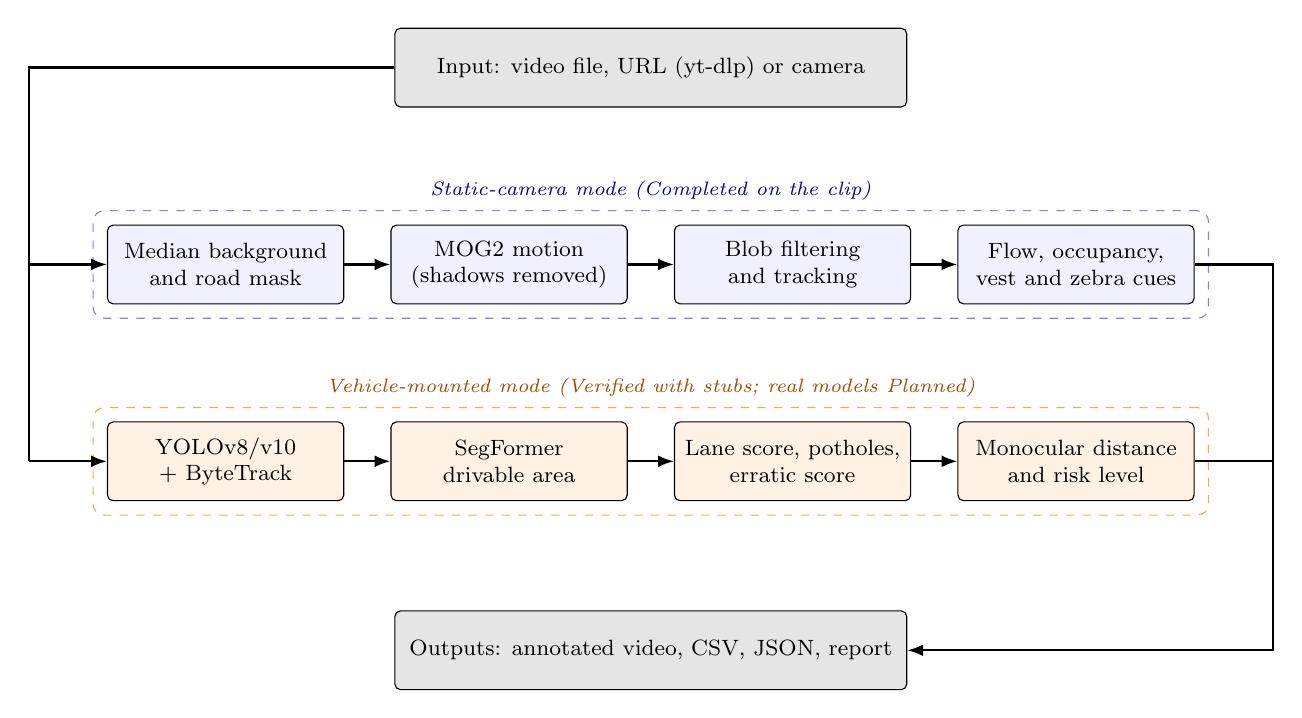
\begin{tikzpicture}[
 box/.style={draw,rounded corners=2pt,align=center,minimum width=3.0cm,minimum height=1.0cm,font=\footnotesize,fill=blue!6},
 io/.style={box,fill=gray!20,minimum width=6.5cm},
 arr/.style={-{Latex[length=2mm]},thick}]
\node[io] (in) at (0,0) {Input: video file, URL (yt-dlp) or camera};
\foreach \x/\n/\t in {-5.4/A1/{Median background\\and road mask},-1.8/A2/{MOG2 motion\\(shadows removed)},1.8/A3/{Blob filtering\\and tracking},5.4/A4/{Flow, occupancy,\\vest and zebra cues}}
  \node[box] (\n) at (\x,-2.5) {\t};
\foreach \x/\n/\t in {-5.4/B1/{YOLOv8/v10\\+ ByteTrack},-1.8/B2/{SegFormer\\drivable area},1.8/B3/{Lane score, potholes,\\erratic score},5.4/B4/{Monocular distance\\and risk level}}
  \node[box,fill=orange!10] (\n) at (\x,-5.0) {\t};
\begin{scope}[on background layer]
\node[draw=blue!50,dashed,rounded corners,fit=(A1)(A4),inner sep=5pt,label={[font=\scriptsize\itshape,text=blue!60!black]above:Static-camera mode (Completed on the clip)}] {};
\node[draw=orange!70,dashed,rounded corners,fit=(B1)(B4),inner sep=5pt,label={[font=\scriptsize\itshape,text=orange!60!black]above:Vehicle-mounted mode (Verified with stubs; real models Planned)}] {};
\end{scope}
\node[io] (out) at (0,-7.4) {Outputs: annotated video, CSV, JSON, report};
\draw[arr] (A1)--(A2); \draw[arr] (A2)--(A3); \draw[arr] (A3)--(A4);
\draw[arr] (B1)--(B2); \draw[arr] (B2)--(B3); \draw[arr] (B3)--(B4);
\draw[arr] (in.west)--(-7.9,0)--(-7.9,-2.5)--(A1.west);
\draw[thick] (-7.9,-2.5)--(-7.9,-5.0); \draw[arr] (-7.9,-5.0)--(B1.west);
\draw[arr] (A4.east)--(7.9,-2.5)--(7.9,-7.4)--(out.east);
\draw[thick] (B4.east)--(7.9,-5.0);
\end{tikzpicture}}
\caption{System architecture.}
\label{fig:arch}
\end{figure}

\noindent\textbf{Folder structure} (the whole project compiles and runs from this layout):
\begin{lstlisting}[language={},numbers=none,basicstyle=\ttfamily\footnotesize]
indian_road_perception_project/
|-- report.tex, report.pdf        this report (numbers auto-filled from generated/)
|-- paper.tex, paper.pdf          research-paper version of the advanced study
|-- Makefile                      make test | experiments | collect | report | all
|-- README.md, requirements*.txt, pyproject.toml
|-- src/irp/
|   |-- common.py                 categories, video I/O, segmenters, lane/pothole, motion, geometry
|   |-- static.py                 static-camera pipeline (resolution-adaptive, executed)
|   |-- quality.py                quality profile, enhancement, stabilisation
|   |-- tracking.py               Kalman + Hungarian tracker
|   |-- flow.py                   gates, headways, bursts
|   |-- robustness.py             degradation study (ffmpeg)
|   |-- bench.py                  tracker benchmark with exact ground truth
|   |-- vehicle.py                vehicle-mounted pipeline (YOLO + SegFormer, injectable)
|   `-- collect.py                results -> LaTeX tables, macros, figures
|-- tests/test_irp.py             unit and integration tests (synthetic, stub models)
|-- data/junction_clip.mp4        junction 1 (1280x720)
|-- data/junction2_360p.mp4       junction 2 (640x360)
|-- results/<run>/                summary.json, params.json, frames.csv, tracks.csv, ...
|-- figures/  generated/          produced by `python -m irp.collect`
\end{lstlisting}

% =====================================================================
\section{Methodology and Essential Equations}
% =====================================================================
\textbf{Static camera.} The background is the temporal median of 60 frames; the road mask is the largest low-saturation, non-dark region below
the far road edge. Motion is segmented with MOG2~\cite{zivkovic2004}, where each pixel is a Gaussian mixture
\begin{equation}
p(\mathbf{x}_t)=\sum_{k=1}^{K}\pi_k\,\mathcal{N}\!\left(\mathbf{x}_t;\boldsymbol\mu_k,\sigma_k^2\mathbf{I}\right),
\end{equation}
with shadow pixels (a darkened background of similar chromaticity) relabelled and discarded. Blobs whose base touches the road are tracked by
nearest-centroid matching; a track is confirmed after $L_{\min}$ frames and 40\,px displacement. Orange hi-vis blobs mark traffic police, and
tracks containing a vest are excluded from traffic statistics.

\textbf{Perspective-normalised size.} For a camera of height $H_c$ over flat ground with horizon row $y_h$, a ground-contact point at row $y_b$ has depth $Z=fH_c/(y_b-y_h)$.
An object of physical size $\sqrt{W_oH_o}$ appears as $\sqrt{wh}=f\sqrt{W_oH_o}/Z$, hence
\begin{equation}
s=\frac{\sqrt{wh}}{y_b-y_h}=\frac{\sqrt{W_oH_o}}{H_c}
\end{equation}
is independent of distance. Relative speed is displacement divided by (median box width $\times$ duration), in body widths per second.

\textbf{Road occupancy} (congestion proxy), with foreground $F_t$, road mask $R$ and its dilation $\mathcal{D}$:
\begin{equation}
O_t=\frac{|F_t\cap\mathcal{D}(R)|}{|R|}.
\end{equation}

\textbf{Vehicle-mounted mode.} Monocular range, with $f=\tfrac{W/2}{\tan(\mathrm{HFOV}/2)}$:
\begin{equation}
d=\frac{f\,H_c}{y_b-y_h}.
\end{equation}
Lane-marking quality from paint fraction $\rho$ and near-vertical Hough segment count $n$: $S=0.5\min(1,40\rho)+0.5\min(1,n/6)$
(\emph{clear} $S>0.6$, \emph{faded} $S>0.25$, else \emph{absent}).
Erratic motion: with lateral step $\delta_t=(x_t-x_{t-1})/w_t$ minus the median over tracks (ego-motion compensation), a user is flagged if
$\delta$ changes sign at least three times with $\overline{|\delta|}>0.05$ over 12 steps, or $\max|\delta|>0.6$.
Risk is \emph{HIGH} if a vulnerable user (two-wheeler, pedestrian, animal) is in the ego corridor with $d<8$\,m, or an erratic user is in the
widened corridor with $d<12$\,m; \emph{MED} if a vulnerable user is in the corridor with $d<20$\,m.
Detector classes are mapped to categories so that COCO and IDD-fine-tuned models both work.

% =====================================================================
\section{Implementation}
% =====================================================================
\begin{table}[H]
\centering
\caption{Modules (complete listings in Appendix~\ref{app:code}).}
\begin{tabular}{@{}lp{11.4cm}@{}}
\toprule
File & Role \\
\midrule
\texttt{common.py} & Category mapping, \texttt{Detection}, video I/O and time windows, URL download, SegFormer and colour-model road segmenters, lane score, pothole heuristic, geometry, \texttt{MotionAnalyzer}. \\
\texttt{static.py} & \texttt{StaticConfig}, \texttt{analyze()}: background, road mask, MOG2, tracker choice, enhancement, stabilisation, police (persistence) and zebra cues, metrics, flow, CSV/JSON/video output. See Section~\ref{sec:advanced} for the v2 modules. \\
\texttt{vehicle.py} & \texttt{VehicleConfig}, \texttt{run()}, \texttt{assess\_risk()}, YOLO adapters; detector and segmenter are injected. \\
\texttt{collect.py} & Reads every \texttt{results/<run>/}, writes \texttt{generated/experiments.tex}, \texttt{generated/macros.tex} and all figures. \\
\texttt{tests/test\_irp.py} & \mTests\ tests (\mTestsStatus): mapping, geometry, lane, pothole, weaving, risk, static pipeline on a synthetic crossing, vehicle pipeline with stub models. \\
\bottomrule
\end{tabular}
\end{table}

\begin{lstlisting}[language={},numbers=none,basicstyle=\ttfamily\footnotesize,caption={Typical commands.}]
pip install -r requirements.txt              # core;  requirements-dl.txt adds torch, ultralytics, transformers, yt-dlp
make test                                    # runs the test-suite, writes results/tests.log
make -j5 experiments                         # runs all experiments in results/
python -m irp.static  --source data/junction_clip.mp4 --out results/main --label "Baseline"
python -m irp.static  --source "<URL>" --out results/road2 --duration 5      # any road via link (needs yt-dlp)
python -m irp.vehicle --source drive.mp4 --out results/drive1                # needs requirements-dl.txt
make collect report                          # regenerate tables, figures, report.pdf
\end{lstlisting}

Environment of the completed runs: Python~3, OpenCV~\mOpenCV, NumPy~\mNumpy, CPU only. The baseline run processed \mFramesAnalysed\ analysed frames
(plus warm-up) of the $1280\times720$ clip at $960\times540$ in \mWall\,s (\mProcFps\ frames/s including video encoding, about 0.6 times real time).

% =====================================================================
\section{Road Users and Hazards}
% =====================================================================
\begin{table}[H]
\centering
\caption{Road-user catalogue. ``In clip'' is from visual inspection of the video, not an automatic classification.}
\small
\begin{tabular}{@{}p{2.6cm}p{3.9cm}p{4.3cm}p{1.5cm}p{1.2cm}@{}}
\toprule
Road user & Typical behaviour & Perception hazard & COCO class & In clip \\
\midrule
Two-wheeler & Filters between vehicles, sudden lateral moves, rides in groups & Small, fast, hidden by larger vehicles; rider and bike must be grouped & Yes (rider = person) & Yes \\
Auto-rickshaw & Abrupt stops, wide turns, passenger loading & No COCO class; confused with car/truck; merges when adjacent & No & Yes \\
Car / MPV & Follows flow, ignores lanes & Few special issues & Yes & Yes \\
Bus & Wide swing, stops mid-road & Large occlusion, merged blobs, wide shadow & Yes & Yes \\
Pedestrian & Crosses anywhere, groups & Partial occlusion, small scale & Yes & Yes (far) \\
Traffic police & Gestures override signals & No class; only the vest cue is detected here & No & Yes (2) \\
Truck, tractor, loaded vehicle & Slow, protruding loads & Unusual shapes & Partly & No \\
Animal (cow, dog) & Stands or sleeps on road & Unpredictable, static clutter & Yes & No \\
Hand-cart, e-rickshaw & Slow, often unlit & No COCO class & No & No \\
\bottomrule
\end{tabular}
\end{table}

\begin{table}[H]
\centering
\caption{Hazard register. Priority is the author's qualitative judgement (likelihood $\times$ perception difficulty), not a measurement.}
\small
\begin{tabular}{@{}l p{3.2cm} p{3.9cm} p{3.4cm} p{1.5cm} c@{}}
\toprule
ID & Hazard & Effect on perception & Mitigation & Evidence & Prio. \\
\midrule
H1 & Sun glare, overexposed asphalt & Paint and colour cues vanish & HDR, exposure control, learned segmentation & Observed & H \\
H2 & Tree and flyover shadows & False motion, holes in road mask & Shadow suppression (quantified in E2) & Observed & H \\
H3 & Side-by-side vehicles & Merged blobs, count errors & Detector with tracking, instance masks & Observed & H \\
H4 & Manual traffic control & Right of way unclear from objects alone & Pose-based gesture model & Observed & H \\
H5 & Bus occlusion & Hidden two-wheelers and pedestrians & Multi-camera or LiDAR, occlusion reasoning & Partly & M \\
H6 & Potholes, speed breakers & Unsafe path, ride harm & Trained pothole model, LiDAR profile & Not in clip & H \\
H7 & Animals on road & Late detection, unpredictable motion & Animal classes, larger margins & Not in clip & M \\
H8 & Night, headlight glare & Low contrast, blooming & Night data, IR or thermal, exposure control & Not in clip & H \\
H9 & Rain, water-logging, dust on lens & Blur, depth misjudged, false road mask & Lens cleaning, wet-road data & Not in clip & M \\
H10 & Wrong-way or lane-cutting riders & Unexpected trajectories & Trajectory anomaly score & Not in clip & H \\
H11 & Open manholes, unmarked speed breakers & Missed road defects & Dedicated detector, map prior & Not in clip & M \\
\bottomrule
\end{tabular}
\end{table}

% =====================================================================
\section{Completed Experiments}\label{sec:completed}
% =====================================================================
All experiments use \texttt{data/junction\_clip.mp4}: \mDuration\,s, $1280\times720$, 30\,fps, fixed camera at a signalised junction under a flyover,
bright sun, two traffic police in the carriageway. No ground truth exists, so all figures are estimates checked by visual inspection.
The first 30 frames (background warm-up) are excluded from occupancy statistics.

\begin{table}[H]
\centering
\caption{Experiment log (auto-generated from \texttt{results/}). T/A = toward/away from camera; Speed in body widths per second.}
\resizebox{\textwidth}{!}{\begin{tabular}{@{}l p{4.6cm} r r c r r l r@{}}
\toprule
Run & Description & Tracks & Police & R$\to$L/L$\to$R/T/A & Occ.\ mean & Occ.\ p95 & Peak (t) & Speed \\
\midrule
main & J1 baseline (greedy tracker) & 39 & 8 & 20/11/5/3 & 9.6\,\% & 20.5\,\% & 26.9\,\% (21.8\,s) & 1.72 \\
a\_kalman & J1 Kalman + Hungarian tracker & 46 & 10 & 23/15/4/4 & 9.6\,\% & 20.5\,\% & 26.9\,\% (21.8\,s) & 1.77 \\
b\_enh & J2 Kalman + denoise + CLAHE & 253 & 3 & 165/77/8/3 & 5.1\,\% & 18.6\,\% & 42.6\,\% (16.6\,s) & 2.42 \\
b\_greedy & J2 greedy tracker & 166 & 3 & 118/45/1/2 & 4.4\,\% & 14.0\,\% & 35.5\,\% (16.7\,s) & 2.21 \\
b\_main & J2 (360p) Kalman tracker, no enhancement & 215 & 3 & 143/65/6/1 & 4.4\,\% & 14.0\,\% & 35.5\,\% (16.7\,s) & 2.35 \\
b\_noshadow & J2 ablation: shadows counted as foreground & 227 & 3 & 151/72/4/0 & 5.9\,\% & 18.9\,\% & 44.3\,\% (16.7\,s) & 2.05 \\
first5s & J1 first 5 s only & 11 & 0 & 5/5/1/0 & 5.7\,\% & 9.6\,\% & 10.4\,\% (1.7\,s) & 1.58 \\
mt20 & J1 min. track length 20 frames & 28 & 7 & 13/10/3/2 & 9.6\,\% & 20.5\,\% & 26.9\,\% (21.8\,s) & 1.54 \\
mt8 & J1 min. track length 8 frames & 43 & 8 & 23/11/5/4 & 9.6\,\% & 20.5\,\% & 26.9\,\% (21.8\,s) & 1.78 \\
noshadow & J1 ablation: shadows counted as foreground & 42 & 9 & 15/18/6/3 & 13.0\,\% & 28.0\,\% & 33.6\,\% (21.7\,s) & 1.70 \\
\bottomrule
\end{tabular}
}
\end{table}

\subsection*{E1: Baseline on the full clip}
\mTracks\ confirmed tracks (\mPolice\ police tracks excluded); direction R$\to$L/L$\to$R/toward/away = \mDirRL/\mDirLR/\mDirTo/\mDirAway;
mean occupancy \pct{\mOccMean}, 95th percentile \pct{\mOccPNN}, peak \pct{\mOccPeak} at \mOccPeakT\,s (a bus crosses with autos and scooters);
median relative speed \mSpeed\ body widths/s; median track duration \mTrackDur\,s; on average \mMeanUsers\ tracked users per frame;
police vest visible in \pct{\mVest} of frames; zebra crossing found at the lower left (\mZebra\ stripe candidates); road covers \pct{\mRoadArea} of the image.

\begin{figure}[H]
\centering
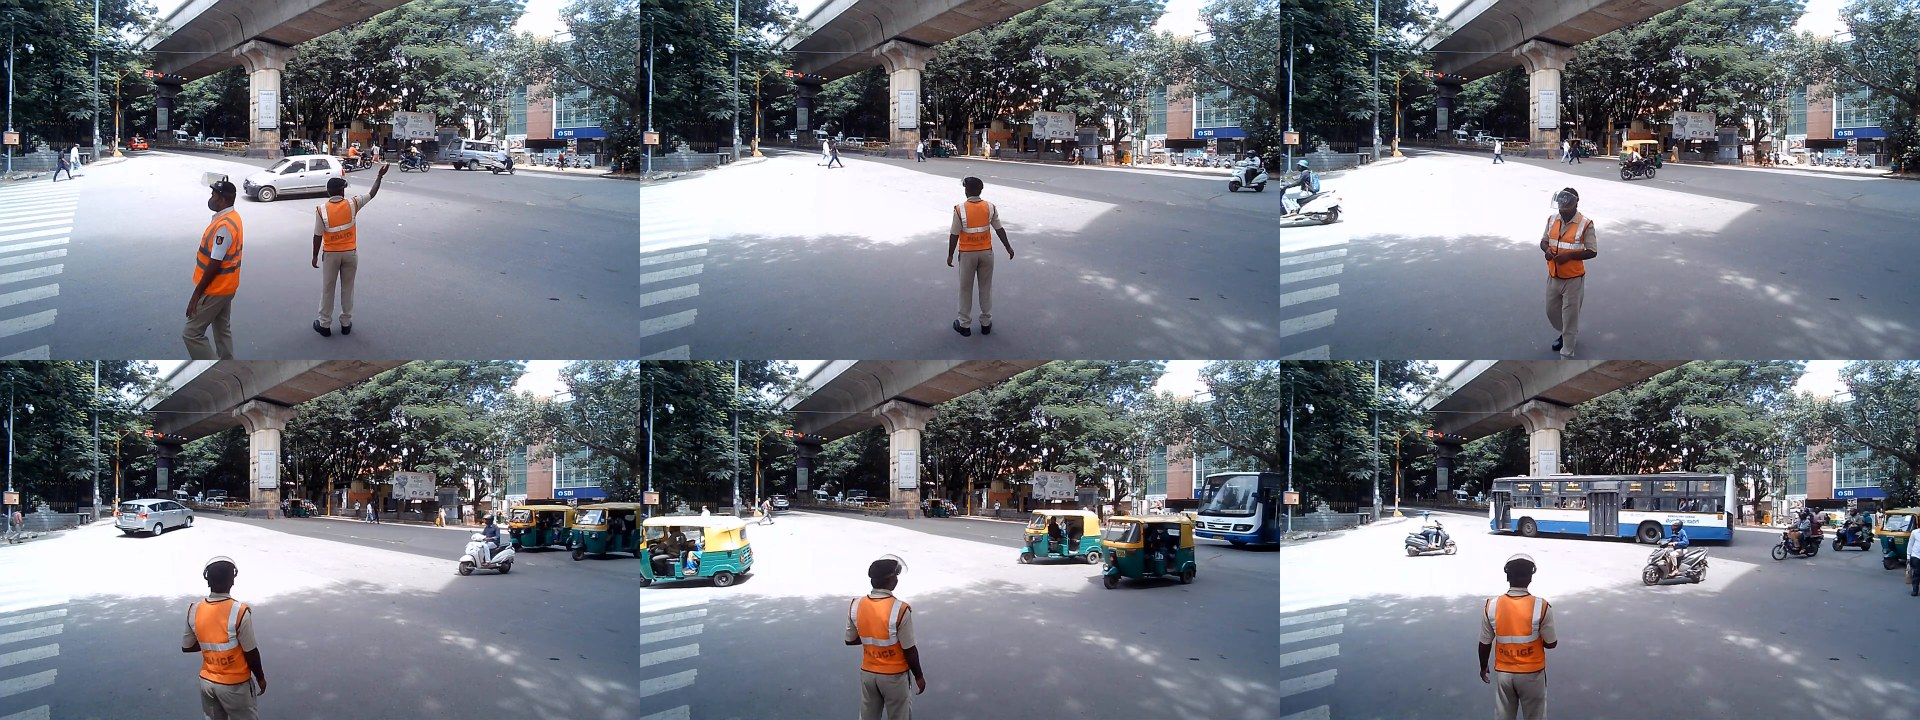
\includegraphics[width=\textwidth]{fig_scene.jpg}
\caption{Frames evenly spaced over the clip: scooters and motorcycles, auto-rickshaws, cars and a bus with two officers.}
\end{figure}
\begin{figure}[H]
\centering
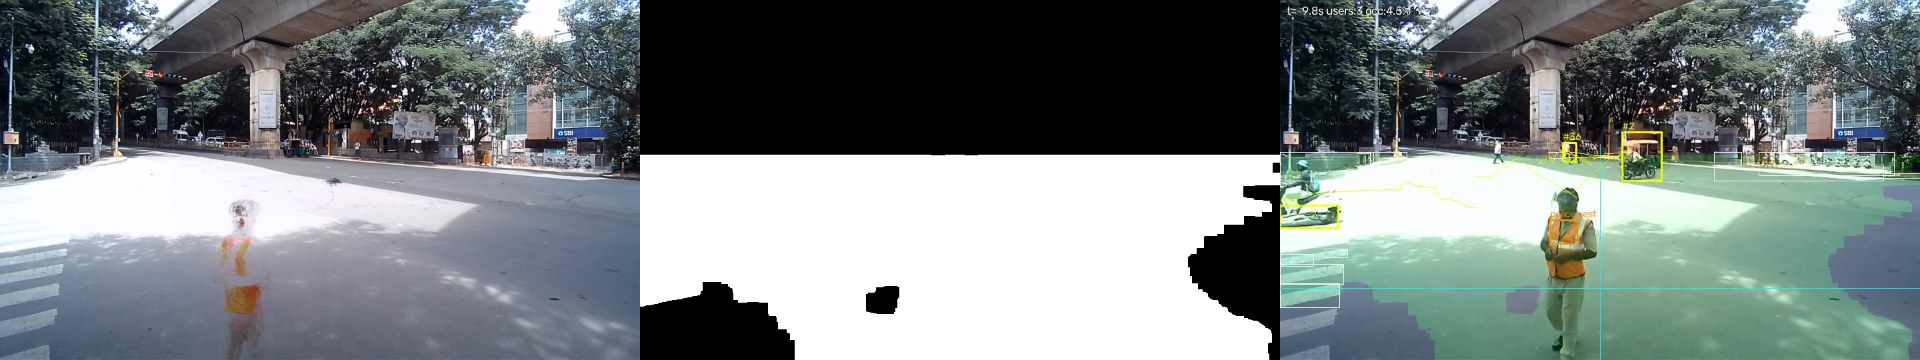
\includegraphics[width=\textwidth]{fig_method.jpg}
\caption{Left: median background (the standing officer is a faint ghost). Centre: road mask. Right: annotated frame (road green, tracks yellow, vests orange, zebra white).}
\end{figure}
\begin{figure}[H]
\centering
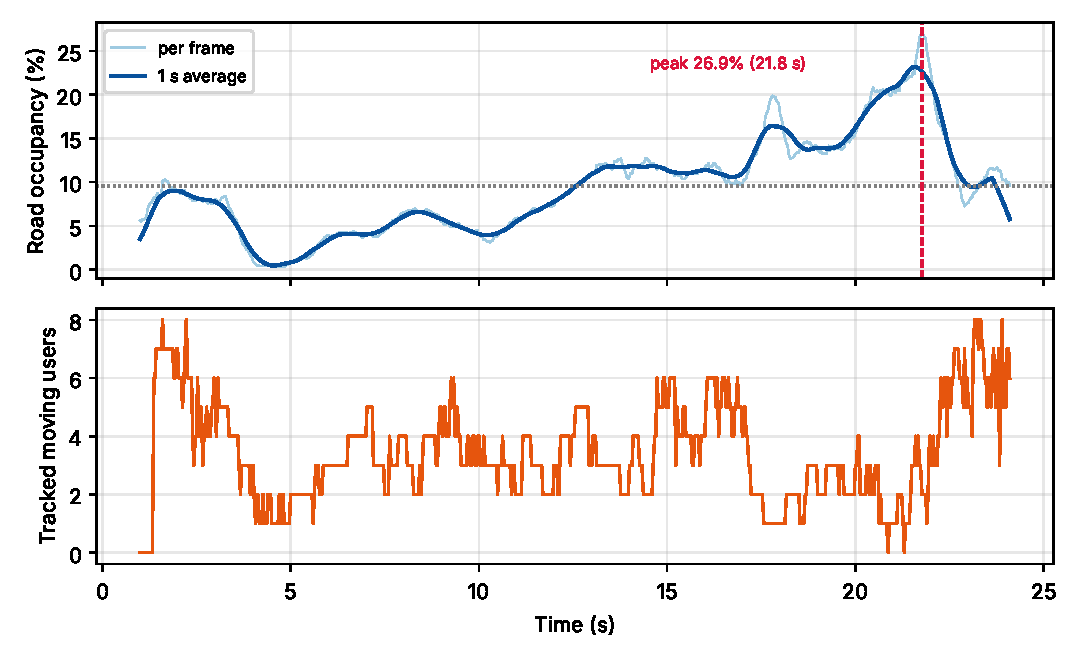
\includegraphics[width=0.92\textwidth]{fig_occupancy.pdf}
\caption{E1: road occupancy (thin line per frame, thick line 1\,s average, dotted line mean) and tracked users per frame.}
\end{figure}
\begin{figure}[H]
\centering
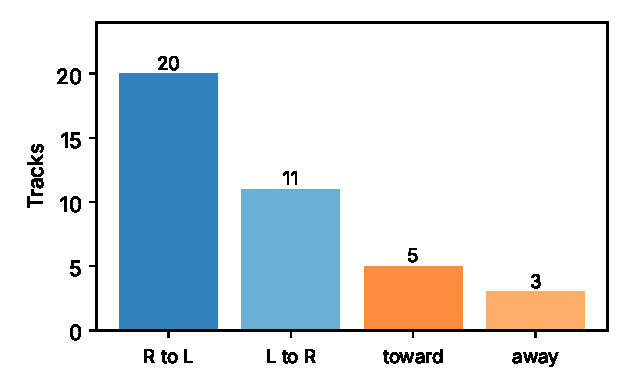
\includegraphics[width=0.5\textwidth]{fig_directions.pdf}\hfill
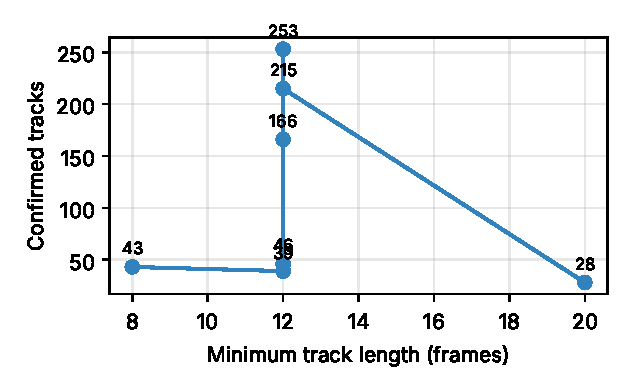
\includegraphics[width=0.48\textwidth]{fig_sensitivity.pdf}
\caption{Left: direction of travel (E1). Right: confirmed tracks versus minimum track length (E3).}
\end{figure}
\begin{figure}[H]
\centering
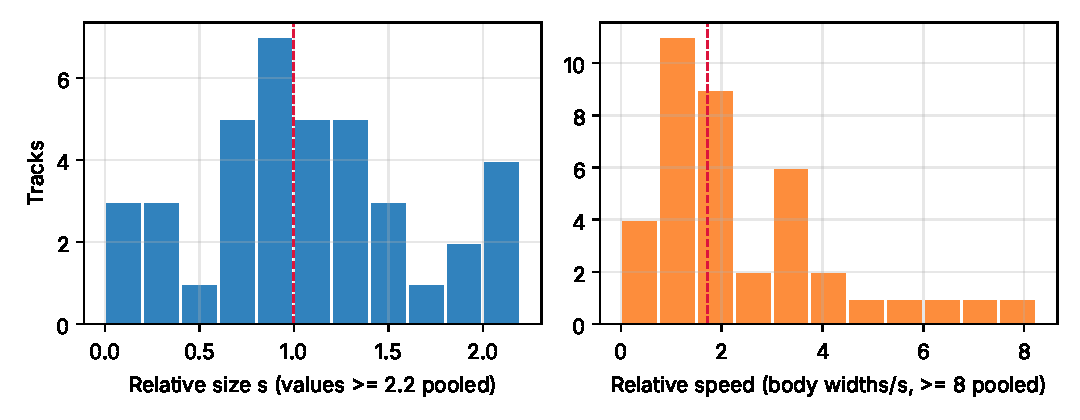
\includegraphics[width=0.95\textwidth]{fig_hist.pdf}
\caption{E1: histograms of relative size $s$ and relative speed; dashed line is the median, overflow is pooled in the last bin.}
\end{figure}
\begin{figure}[H]
\centering
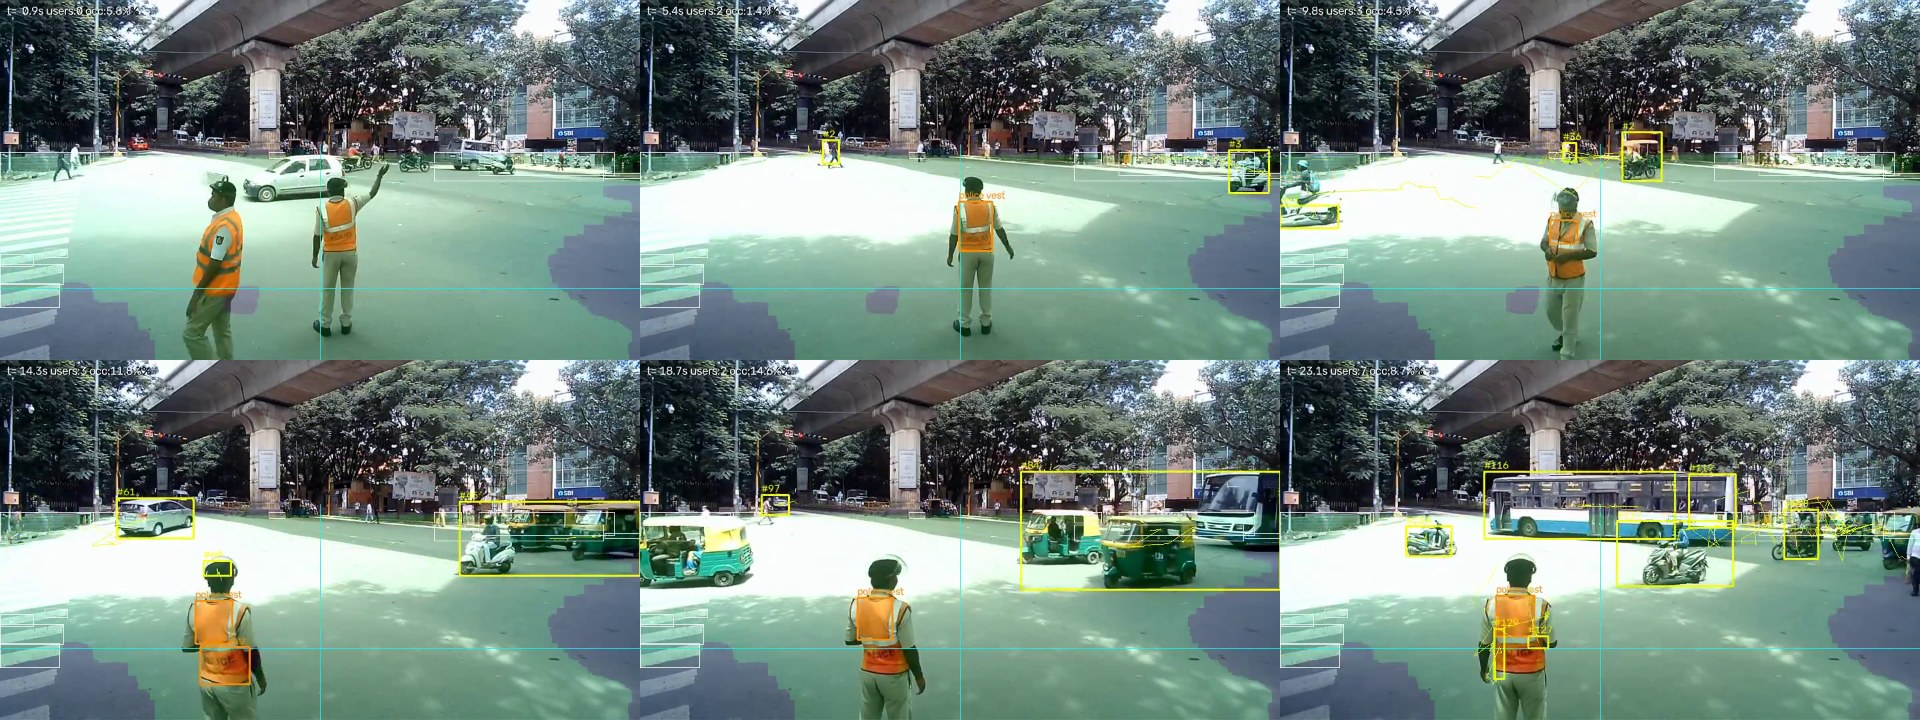
\includegraphics[width=\textwidth]{fig_annotated.jpg}
\caption{Annotated frames from \texttt{results/main/annotated.mp4}. Officers are excluded from traffic counts.}
\end{figure}

\textbf{Observations (visual inspection of the annotated video).}
Autos, scooters, the car and the bus are boxed and followed in most frames. Failure cases: vehicles side by side merge into one box;
the lower body of a walking officer (no vest in the box) is sometimes tracked as traffic; deep shadow on the right of the carriageway is missing from the road mask.

\subsection*{E2: Shadow-suppression ablation}
With MOG2 shadow detection off, mean occupancy rises from \pct{\mOccMean} to \pct{\mNSOccMean} (+\mShadowGainPP\ percentage points, +\pct{\mShadowGainRel} relative),
the 95th percentile from \pct{\mOccPNN} to \pct{\mNSOccPNN}, and the peak from \pct{\mOccPeak} to \pct{\mNSOccPeak}; confirmed tracks change from \mTracks\ to \mNSTracks\
and police tracks from \mPolice\ to \mNSPolice. The peak time is unchanged, but the direction split shifts (Table above), so direction counts are sensitive to foreground quality.

\begin{figure}[H]
\centering
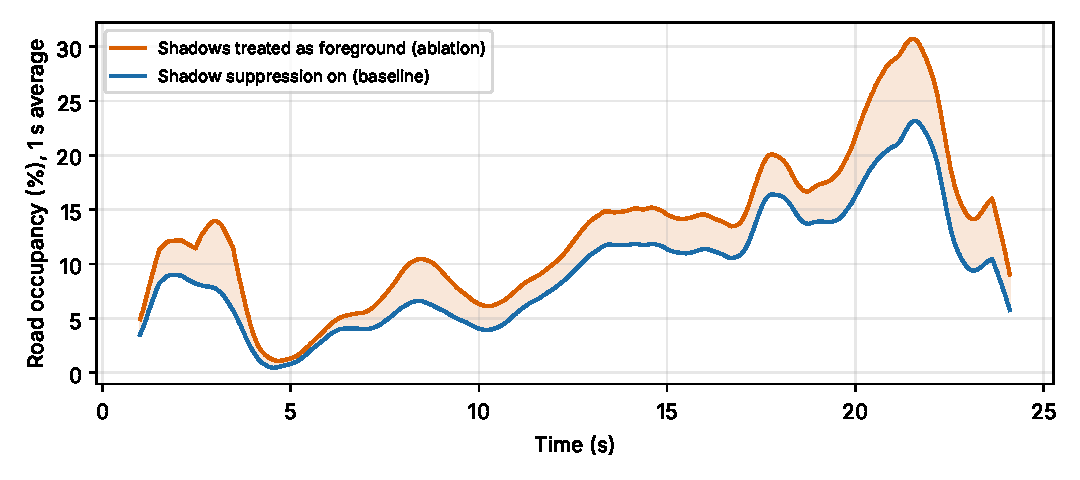
\includegraphics[width=0.9\textwidth]{fig_ablation.pdf}
\caption{E2: occupancy with and without shadow suppression; the shaded area is false occupancy attributable to shadows.}
\end{figure}

\subsection*{E3: Sensitivity to minimum track length}
Lowering $L_{\min}$ to \mMtLowL\ frames gives \mMtLowTracks\ tracks, raising it to \mMtHighL\ gives \mMtHighTracks\ (baseline \mTracks). Occupancy is identical in all three
runs because it does not depend on tracking. Track counts should therefore be read as estimates with roughly $\pm25\,\%$ uncertainty.

\subsection*{E4: First five seconds}
A \mFiveDur\,s window (frames 0--150; the first second is warm-up) gives \mFiveTracks\ confirmed tracks, mean occupancy \pct{\mFiveOccMean}, peak \pct{\mFiveOccPeak},
and police vests visible in \pct{\mFiveVest} of frames. This segment is quiet compared with the end of the clip, where the bus crosses.

\subsection*{T1: Automated tests (Verified)}
\mTests\ tests, \mTestsStatus\ (\texttt{results/tests.log}). They cover mapping, geometry, lane score (paint versus none), pothole candidate, weaving versus steady
tracks, risk levels, the static pipeline on a synthetic crossing object, and the full vehicle pipeline with stub models (risk HIGH for a near pedestrian, weaving
two-wheeler flagged). These tests verify the code paths; they are not evidence of accuracy on real roads.

% =====================================================================
\section{Advanced Study on Low-Quality Video}\label{sec:advanced}
% =====================================================================
Version~2 targets low-quality fixed-camera footage and research-grade evidence. A paper-style write-up is in \texttt{paper.pdf}; this section summarises it.
New modules: \texttt{quality.py} (quality profile, enhancement, stabilisation), \texttt{tracking.py} (Kalman + Hungarian), \texttt{flow.py} (gates, headways, bursts),
\texttt{robustness.py} (degradation study), \texttt{bench.py} (tracker benchmark with exact ground truth). All pixel parameters scale with the processing width, and a persistence rule
(vests must stay in place for 2\,s) stops orange vehicles being counted as police. \textbf{Evidence level: Completed} (real clips, simulation, degradation); no human labels exist for the real clips.

\subsection*{Q1: Video-quality profile of both clips}
\begin{table}[H]
\centering
\caption{Quality profile (sharpness is scene-dependent).}
\small
\resizebox{0.9\textwidth}{!}{\begin{tabular}{@{}lrr@{}}
\toprule
Measure & junction1\_720p & junction2\_360p \\
\midrule
Resolution & 1280$\times$720 & 640$\times$360 \\
Duration (s) & 24.1 & 118.8 \\
Bits per pixel (file size) & 0.082 & 0.077 \\
Noise $\sigma$ (grey levels) & 2.10 & 3.03 \\
Blockiness (1 = none) & 1.072 & 1.069 \\
Sharpness (Laplacian variance at 640 px) & 5081 & 2281 \\
Overexposed pixels (\%) & 7.9 & 11.0 \\
Mean brightness / contrast & 120 / 69 & 123 / 75 \\
Inter-frame jitter, RMS (px) & 0.070 & 0.017 \\
Flags & glare\_or\_clipping & low\_resolution, noisy, glare\_or\_clipping \\
\bottomrule
\end{tabular}
}
\end{table}
Clip~B ($640\times360$) is noisier (noise $\sigma$ \mQBNoise\ versus \mQANoise); both clips have strong glare and negligible jitter (RMS \mQBJitter\ and \mQAJitter\,px), so stabilisation is not needed here.

\subsection*{Q2: Tracker benchmark (simulated, exact ground truth)}
\begin{table}[H]
\centering
\caption{Greedy versus Kalman + Hungarian tracking (mean$\pm$std over \mBenchSeeds\ seeds).}
\small
\resizebox{\textwidth}{!}{\begin{tabular}{@{}llccccc@{}}
\toprule
Scenario & Tracker & Fragments/object & ID switches & Purity & Count ratio & False tracks \\
\midrule
clean & greedy & 1.55$\pm$0.45 & 5.7$\pm$5.1 & 0.881$\pm$0.102 & 0.96$\pm$0.06 & 0.0$\pm$0.0 \\
 & kalman & 1.00$\pm$0.00 & 0.0$\pm$0.0 & 0.998$\pm$0.009 & 0.99$\pm$0.03 & 0.0$\pm$0.0 \\
missed & greedy & 3.29$\pm$0.59 & 29.0$\pm$10.8 & 0.753$\pm$0.074 & 1.12$\pm$0.10 & 0.0$\pm$0.0 \\
 & kalman & 1.23$\pm$0.27 & 2.2$\pm$2.6 & 0.983$\pm$0.023 & 1.04$\pm$0.09 & 0.0$\pm$0.0 \\
occluded & greedy & 4.10$\pm$0.93 & 44.4$\pm$19.4 & 0.718$\pm$0.081 & 1.24$\pm$0.17 & 0.0$\pm$0.0 \\
 & kalman & 1.51$\pm$0.35 & 6.3$\pm$5.9 & 0.938$\pm$0.053 & 1.11$\pm$0.13 & 0.0$\pm$0.0 \\
dense & greedy & 7.63$\pm$0.74 & 222.1$\pm$35.6 & 0.530$\pm$0.041 & 1.22$\pm$0.10 & 0.0$\pm$0.0 \\
 & kalman & 2.12$\pm$0.41 & 30.4$\pm$11.3 & 0.881$\pm$0.045 & 1.14$\pm$0.10 & 0.0$\pm$0.0 \\
\bottomrule
\end{tabular}
}
\end{table}
In dense traffic Kalman tracking reduces identity switches from \mBenchGDenseIdsw\ to \mBenchKDenseIdsw\ and fragments per object from \mBenchGDenseFrag\ to \mBenchKDenseFrag.
\begin{figure}[H]
\centering
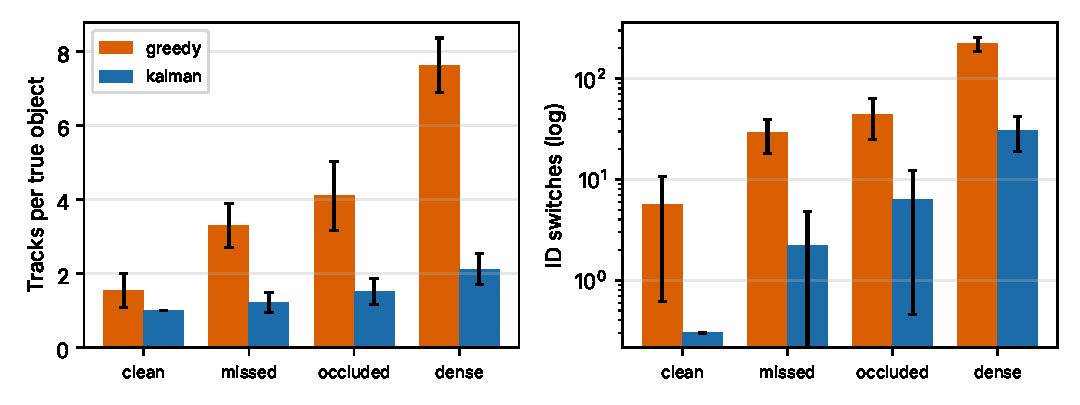
\includegraphics[width=0.85\textwidth]{fig_benchmark.pdf}
\caption{Fragmentation and identity switches per scenario.}
\end{figure}

\subsection*{Q3: Degradation study (reference-based)}
Junction~1 was degraded in \mRobNConds\ ways (resolution, blur, noise, compression, combined) and compared with the original analysis (\mRobRefTracks\ tracks, mean occupancy \mRobRefOcc\,\%).
Occupancy correlation stays between \mRobMinRNone\ and \mRobMaxR\ without enhancement; track counts deviate by up to \mRobMaxTrackDev\,\%. Enhancement lowers the occupancy error in \mRobEnhBetter\ of \mRobNConds\ conditions but not on average
(\mRobMaeNone\ versus \mRobMaeFull\,pp), and hurts at $320\times180$.
\begin{table}[H]
\centering
\caption{Agreement of degraded versions with the reference (see \texttt{paper.pdf} for definitions).}
\small
\resizebox{\textwidth}{!}{\begin{tabular}{@{}lcccccccc@{}}
\toprule
 & \multicolumn{2}{c}{Occupancy $r$} & \multicolumn{2}{c}{MAE (pp)} & \multicolumn{2}{c}{Mean ratio} & \multicolumn{2}{c}{Track ratio} \\
Condition & none & enh. & none & enh. & none & enh. & none & enh. \\
\midrule
res360 & 0.994 & 0.990 & 1.59 & 1.05 & 0.83 & 0.89 & 1.28 & 1.13 \\
res270 & 0.987 & 0.983 & 1.92 & 1.43 & 0.80 & 0.85 & 1.04 & 1.22 \\
res180 & 0.982 & 0.975 & 3.16 & 4.29 & 1.33 & 1.45 & 0.78 & 0.83 \\
blur2 & 0.998 & 0.993 & 0.38 & 0.84 & 0.97 & 1.07 & 1.02 & 1.13 \\
noise10 & 0.995 & 0.995 & 1.13 & 0.43 & 0.88 & 0.98 & 0.91 & 1.11 \\
crf35 & 0.997 & 0.991 & 0.32 & 0.96 & 1.00 & 1.09 & 1.22 & 1.06 \\
crf45 & 0.964 & 0.964 & 1.59 & 1.55 & 1.12 & 1.13 & 1.37 & 1.20 \\
combo & 0.964 & 0.963 & 1.71 & 1.41 & 0.86 & 0.91 & 1.13 & 1.24 \\
\bottomrule
\end{tabular}
}
\end{table}
\begin{figure}[H]
\centering
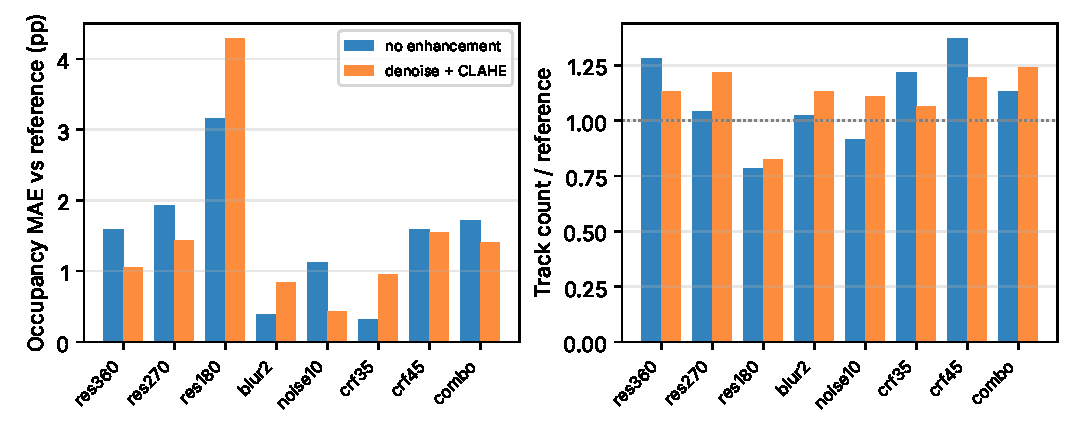
\includegraphics[width=0.9\textwidth]{fig_robustness.pdf}
\caption{Occupancy error and track-count ratio per degradation condition.}
\end{figure}

\subsection*{Q4: Junction 2 (360p, \mBDuration\,s)}
\mBTracks\ tracks (\mBDirRL\ right-to-left, \mBDirLR\ left-to-right); mean occupancy \mBOccMean\,\% (peak \mBOccPeak\,\% at \mBOccPeakT\,s); mid-gate crossings \mBCrossVRL\ R$\to$L and \mBCrossVLR\ L$\to$R, median headway \mBHeadMed\,s;
\mBBurstN\ traffic bursts (mean interval \mBBurstInt\,s, CV \mBBurstCV; too few to claim a signal cycle). Shadow suppression removes \mBNSGain\,pp (+\mBNSGainRel\,\% relative) of false occupancy; greedy, Kalman and enhanced runs give
\mBGreedyTracks, \mBTracks\ and \mBEnhTracks\ tracks (no labels: which is closest to the truth is unknown).
\begin{figure}[H]
\centering
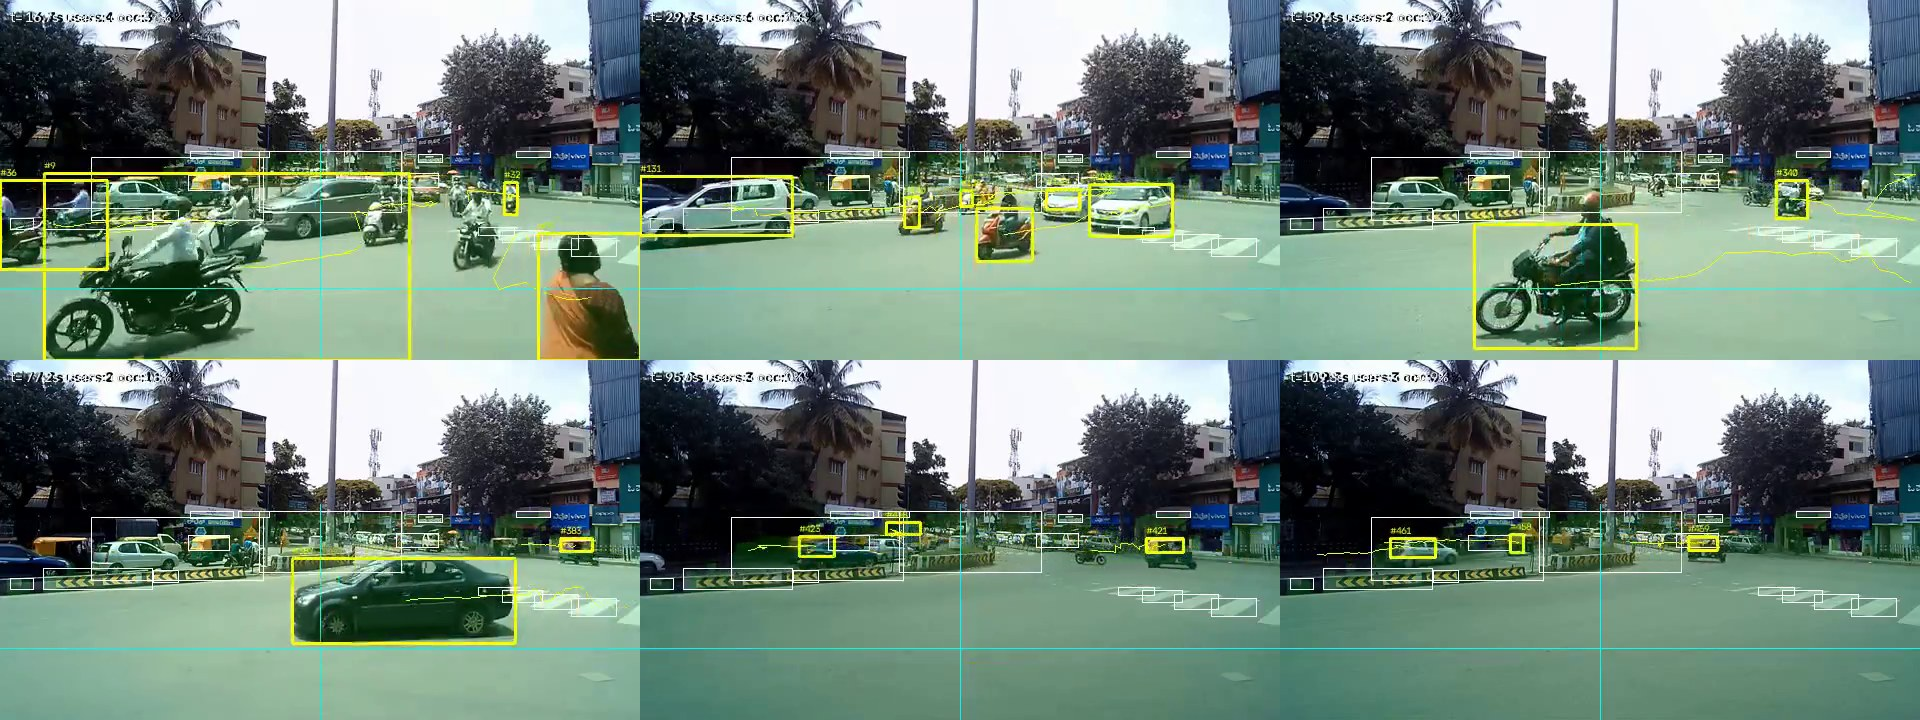
\includegraphics[width=\textwidth]{figB_annotated.jpg}
\caption{Junction~2, annotated frames. Large boxes may contain several adjacent riders.}
\end{figure}
\begin{figure}[H]
\centering
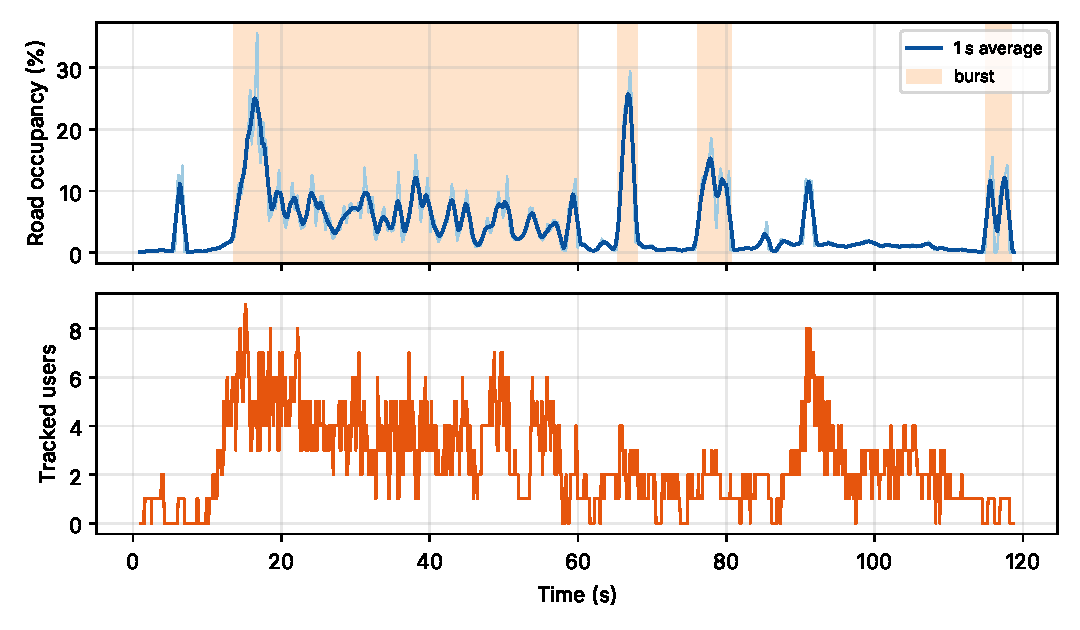
\includegraphics[width=0.9\textwidth]{figB_occupancy.pdf}
\caption{Junction~2: road occupancy with bursts shaded, and tracked users.}
\end{figure}
\begin{table}[H]
\centering
\caption{Junction~2 gate crossings and headways.}
\small
\resizebox{0.9\textwidth}{!}{\begin{tabular}{@{}lllrrrr@{}}
\toprule
Gate & Direction & Crossings & \multicolumn{4}{c}{Headway, all directions (s)} \\
 & & & n & mean & median & p90 \\
\midrule
mid-vertical &  & L->R: 8, R->L: 89 & 97 & 1.16 & 0.44 & 1.85 \\
near-horizontal &  & away: 15, toward: 40 & 55 & 1.17 & 0.59 & 1.95 \\
\bottomrule
\end{tabular}
}
\end{table}
\textbf{Caveats.} The police-vest cue still fires in \mBVest\,\% of junction-2 frames (no police visible; source not verified); the zebra detector also responds to median markings; bursts and counts are estimates without ground truth.

% =====================================================================
\section{Autonomy Stack and Dataset Toolkit (v3)}\label{sec:v3}
% =====================================================================
Version~3 turns the toolkit into one modular code base for any footage from a vehicle camera: the dataset package \texttt{iscvd}
(loaders for IDD, KITTI, BDD100K, Cityscapes, YOLO, COCO, folders and video; unified taxonomy; metrics; benchmark harness; export) and the stack \texttt{irp}
(input handling, ego-motion, detection, tracking, road and lane understanding, intent, forecasting, behaviour planning, MPC/LQR control, a safety supervisor, a closed-loop simulator and a comparison-video generator).
Architecture and extension points are in \texttt{docs/ARCHITECTURE.md}; the publication plan is in \texttt{research\_plan.pdf}.
\textbf{Evidence levels:} \emph{Completed} = executed on the real clips; \emph{Simulation} = closed-loop simulator; \emph{Verified} = tests on synthetic scenes or fixtures; \emph{Not run} = needs data or a GPU.

\begin{table}[H]
\centering\small
\caption{v3 modules and what has been demonstrated. Test count: \mTests\ (\mTestsStatus).}
\begin{tabular}{@{}p{3.4cm}p{7.6cm}p{3.6cm}@{}}
\toprule
Module & Function & Evidence \\
\midrule
\texttt{iscvd} & Loaders, unified taxonomy, AP/mIoU/PQ/MOT/lane/ADE metrics, stats, YOLO/COCO export, benchmark & Verified (fixtures); real IDD/US data not run \\
\texttt{sources}, \texttt{camera} & Any video/image/folder/URL input; ego-motion, horizon, moving-camera check & Verified; 2 real fixed clips \\
\texttt{lanes}, \texttt{road} & BEV lane detection with free-space fallback; road, free space, panoptic fusion & Verified (synthetic) \\
\texttt{detect}, \texttt{tracking} & YOLO / ONNX / motion fallback; Kalman + Hungarian & Verified; YOLO/ONNX weights not run \\
\texttt{predict}, \texttt{intent} & NumPy LSTM forecaster (exact BPTT), HMM intent & Completed (real tracks); intent simulated \\
\texttt{plan}, \texttt{control} & FSM and Q-learning; LQR and MPC & Simulation \\
\texttt{safety}, \texttt{sim} & Independent supervisor and closed-loop benchmark with faults & Simulation \\
\texttt{pipeline}, \texttt{compare} & Unified per-frame pipeline and single comparison video & Completed (demo on 2 clips) \\
\bottomrule
\end{tabular}
\end{table}

\subsection*{Trajectory forecasting on real tracks (Completed)}
Windows of 4 observed and 5 predicted steps (3-frame spacing) from blob-tracker trajectories, split by track. The LSTM reaches ADE \vFcHeldAdeLstm\ body widths against \vFcHeldAdeCv\ for constant velocity on held-out tracks
(\vFcHeldGain\,\% lower; track-bootstrap 95\,\% CI of the paired difference \vFcHeldCiLo\ to \vFcHeldCiHi, \vFcHeldTracks\ tracks) and \vFcCrossAdeLstm\ against \vFcCrossAdeCv\ when trained on junction~2 and tested on junction~1
(CI \vFcCrossCiLo\ to \vFcCrossCiHi, \vFcCrossTracks\ tracks). Gradients agree with finite differences (relative error below $10^{-5}$ in the tests). Small data and blob tracks (not human labels) limit the strength of this evidence.
\begin{table}[H]
\centering\small
\caption{Forecasting errors in body widths (bw) and pixels at 960\,px width.}
\resizebox{\textwidth}{!}{\begin{tabular}{@{}llccccc@{}}
\toprule
Test set & Model & ADE (bw) & FDE (bw) & ADE (px@960) & FDE (px@960) & $\Delta$ADE vs CV [95\% CI] \\
\midrule
held-out tracks (26 tracks) & zero velocity & 0.933 & 1.585 & 72.8 & 123.4 &  \\
 & const. vel. (last) & 0.420 & 0.738 & 32.8 & 57.5 &  \\
 & const. vel. (mean) & 0.422 & 0.740 & 33.2 & 57.6 &  \\
 & ridge regression & 0.398 & 0.666 & 32.5 & 55.4 &  \\
 & LSTM (3-seed ensemble) & 0.342 & 0.569 & 28.9 & 49.0 & -0.155\,\ldots\,-0.025 \\
\midrule
cross-scene (36 tracks) & zero velocity & 0.764 & 1.199 & 38.9 & 61.2 &  \\
 & const. vel. (last) & 0.726 & 1.167 & 35.1 & 56.7 &  \\
 & const. vel. (mean) & 0.606 & 0.948 & 28.4 & 44.5 &  \\
 & ridge regression & 0.554 & 0.858 & 27.2 & 42.3 &  \\
 & LSTM (3-seed ensemble) & 0.507 & 0.780 & 25.5 & 40.2 & -0.174\,\ldots\,-0.043 \\
\bottomrule
\end{tabular}
}
\end{table}
\begin{figure}[H]
\centering
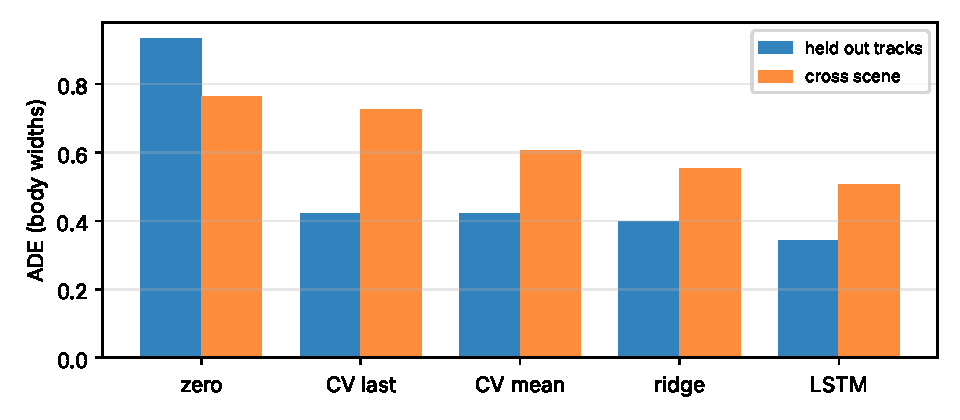
\includegraphics[width=0.6\textwidth]{fig_v3_forecast.pdf}
\caption{ADE of the forecasters on held-out tracks and on the other scene.}
\end{figure}

\subsection*{Closed-loop planning and control (Simulation)}
Five scripted Indian-flavoured scenarios (crossing pedestrian, auto cut-in, weaving two-wheeler, stopped vehicle, braking lead car), 20 seeds each (\vSimEpisodes\ episodes per stack). The Q-learning planner was trained for \vRlEpisodes\ episodes (\vRlSeconds\,s, \vRlStates\ visited states).
MPC adds obstacle-aware braking but costs about \vMpcSolve\,ms per solve on one CPU core. Chunk-merged medians are episode-weighted averages of per-chunk medians. Simulation only: agent behaviour is scripted.
\begin{table}[H]
\centering\small
\caption{Closed-loop results (simulation).}
\resizebox{\textwidth}{!}{\begin{tabular}{@{}lccccccc@{}}
\toprule
Stack & Episodes & Collision rate & Min gap (m) & Min TTC (s) & Jerk (m/s$^3$) & Progress (m) & MPC solve (ms) \\
\midrule
fsm+lqr (no intent) & 100 & 0.03 & 1.41 & 3.40 & 4.71 & 105.2 & -- \\
fsm+lqr+intent & 100 & 0.03 & 1.41 & 4.79 & 5.13 & 76.6 & -- \\
rl+lqr+intent & 100 & 0.01 & 14.01 & 6.10 & 8.88 & 57.7 & -- \\
fsm+mpc+intent & 100 & 0.00 & 5.68 & 8.24 & 4.86 & 75.5 & 49 \\
\bottomrule
\end{tabular}
}
\end{table}

\subsection*{Redundancy under fault injection (Simulation)}
Silent perception faults (empty or frozen world, NaNs), a crash and a latency stall were injected at about 3\,s for 3\,s into FSM+LQR (20 seeds $\times$ 5 scenarios per cell). The supervisor uses an independent range sensor and a fallback controller.
Collisions under dropout fall from \vFaultDropoutPrim\ to \vFaultDropoutSup, under freeze from \vFaultFreezePrim\ to \vFaultFreezeSup, and under NaN from \vFaultNanPrim\ to \vFaultNanSup; the cost is availability: after a crash the vehicle is in fallback \vFaultCrashFallback\ of the time (latched safe stop).
\begin{table}[H]
\centering\small
\caption{Fault injection: collision rate and share of time in fallback.}
\begin{tabular}{@{}lcccc@{}}
\toprule
Fault & \multicolumn{2}{c}{Collision rate} & \multicolumn{2}{c}{Time in fallback} \\
 & primary only & + supervisor & primary only & + supervisor \\
\midrule
none & 0.03 & 0.01 & 0.00 & 0.00 \\
dropout & 0.15 & 0.03 & 0.00 & 0.02 \\
freeze & 0.09 & 0.01 & 0.00 & 0.01 \\
nan & 0.15 & 0.03 & 0.00 & 0.02 \\
crash & 0.06 & 0.01 & 0.00 & 0.75 \\
stall & 0.03 & 0.01 & 0.00 & 0.75 \\
\bottomrule
\end{tabular}

\end{table}
\begin{figure}[H]
\centering
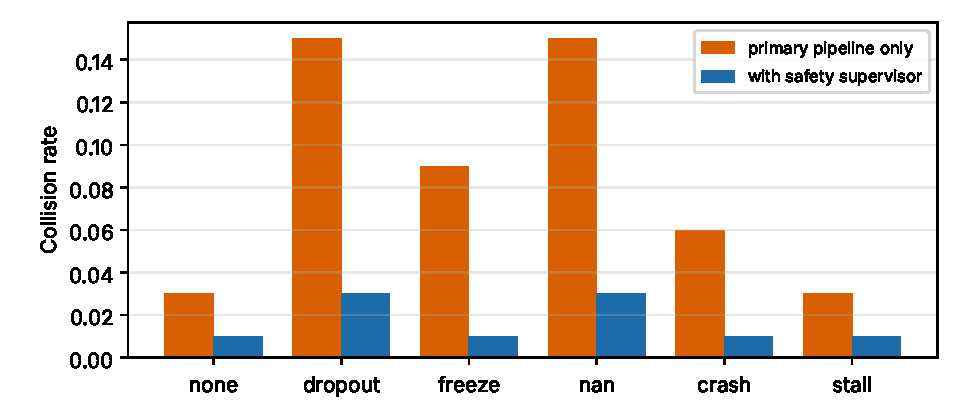
\includegraphics[width=0.6\textwidth]{fig_v3_faults.pdf}
\caption{Collision rate with and without the supervisor.}
\end{figure}

\subsection*{CPU runtime (Completed, no deep model)}
Per-stage latency of the vehicle-mode pipeline on the real 720p clip, one CPU core (\vRtDevice): \vRtFpsLow\ to \vRtFpsHigh\ fps depending on width; lane detection is about \vRtLane\,ms regardless of resolution. GPU numbers were not measured (no GPU available).
\begin{table}[H]
\centering\small
\caption{Mean latency per stage (ms).}
\resizebox{\textwidth}{!}{\begin{tabular}{@{}lccccccccc@{}}
\toprule
Width & ego & detect & track & road & lane & scene & render & total (ms) & fps \\
\midrule
320 & 4.6 & 0.6 & 0.4 & 2.7 & 15.5 & 0.8 & 2.6 & 27.3 & 36.7 \\
480 & 4.8 & 0.8 & 0.4 & 2.4 & 13.1 & 0.9 & 2.9 & 25.2 & 39.7 \\
640 & 5.7 & 0.8 & 0.4 & 4.5 & 13.8 & 1.2 & 4.9 & 31.3 & 32.0 \\
960 & 7.6 & 0.9 & 0.3 & 9.8 & 14.2 & 1.9 & 10.1 & 44.9 & 22.3 \\
\bottomrule
\end{tabular}
}
\end{table}

\subsection*{Synthetic checks (Verified)}
Scenes with exact ground truth confirm the geometry and logic: lane F1 and ego-offset error below, road IoU \vSynRoadIou, and the motion-based fallback detector finds the moving object in a fraction \vSynMotionHit\ of frames but produces \vSynMotionFp\ false boxes per frame on dashed lane paint.
It is a fallback, not a replacement for a trained detector. These numbers say nothing about accuracy on real Indian roads.
\begin{table}[H]
\centering\small
\caption{Lane detection on synthetic scenes.}
\begin{tabular}{@{}lccc@{}}
\toprule
Synthetic lane scene & F1 & Ego-offset error (m) & Path source \\
\midrule
straight & 1.00 & 0.033 & markings \\
curved (c=0.002) & 1.00 & 0.057 & markings \\
ego offset 0.5 m & 1.00 & 0.033 & markings \\
faded paint (25\%) & 1.00 & 0.033 & markings \\
glare & 1.00 & 0.033 & markings \\
noise sigma 8 & 1.00 & 0.033 & markings \\
no paint + free-space fallback & 0.00 & 0.028 & freespace \\
\bottomrule
\end{tabular}

\end{table}

\subsection*{Comparison video (Completed as a tool)}
\texttt{python -m irp.compare} renders one video with both sources side by side (detections and tracks, road, lanes, bird's-eye inset, per-side performance bar) and a final summary card; with labelled datasets it also shows the running detection AP50.
The delivered demo (\texttt{results/compare/comparison.mp4}) uses two Indian fixed-camera clips, so the lane panel misreads zebra stripes: it demonstrates the layout, not an Indian-versus-US result. That comparison needs IDD and a US dataset (plan: \texttt{research\_plan.pdf}).

\subsection*{Not run in this environment}
Learned detectors, segmenters and panoptic networks (no PyTorch, weights or GPU); the Indian-versus-US benchmark (no IDD, KITTI or BDD100K files); validation on footage from a moving vehicle (none was available: moving-camera detection and ego-motion are verified on synthetic drives only); GPU timing; deep reinforcement learning.

% =====================================================================
\section{Planned This Week (Not Yet Run)}\label{sec:planned}
% =====================================================================
Targets below are goals, not results. When an experiment is completed, move its row to Section~\ref{sec:completed}.

\begin{table}[H]
\centering
\small
\caption{Experiments planned for this week.}
\begin{tabular}{@{}l p{4.6cm} p{3.4cm} p{3.4cm} l@{}}
\toprule
ID & Experiment & Metric & Target & Status \\
\midrule
P1 & Run \texttt{irp.vehicle} with YOLOv8n and SegFormer-b0 on forward-facing Indian drive footage & Completes without error; class histogram, risk frames, fps & Report generated; fps recorded & Planned \\
P2 & Hand-label 100 frames of the junction clip (boxes of road users) & Counting error, MOTA/IDF1 of blob tracker & Quantify the $\pm25\,\%$ estimate & Planned \\
P3 & Compare YOLOv8 tracking with the blob tracker on the same clip & Count and direction agreement & Agreement $\ge 80\,\%$ & Planned \\
P4 & Two more Indian road clips via link with the same scripts & Occupancy, flow, vest fraction across scenes & Table of 3+ scenes & Planned \\
P5 & Sweep \texttt{mog\_var\_threshold} $\in\{16,25,36,50\}$ and horizon $\in\{0.40,0.43,0.46\}$ & Occupancy mean, tracks & Parameter-stability range & Planned \\
P6 & Evaluate the pothole heuristic on 50 labelled forward-facing frames & Precision, recall & Documented false-positive rate & Planned \\
\bottomrule
\end{tabular}
\end{table}

% =====================================================================
\section{Future Experiments, Improvements and Additional Observations}
% =====================================================================
\subsection{Hazard-driven experiments}
\begin{itemize}
\item \textbf{Night and rain (H8, H9):} collect or find clips; measure road-mask coverage, detection recall and lane-score drift against daytime baselines.
\item \textbf{Potholes and speed breakers (H6, H11):} train a detector or segmenter; fuse LiDAR range profile; report precision/recall per surface type.
\item \textbf{Animals (H7):} test cow and dog classes from COCO, then IDD fine-tuning; measure first-detection distance.
\item \textbf{Wrong-way and lane-cutting (H10):} trajectory-anomaly score from track histories; evaluate on labelled events.
\item \textbf{Occlusion (H5):} measure track loss while a bus passes; test re-identification.
\end{itemize}

\subsection{Improvements}
\begin{itemize}
\item Fine-tune YOLOv8/v10 on IDD with extra classes (e-rickshaw, hand-cart, tractor, cattle); fine-tune SegFormer with a drivable/fallback label set.
\item Replace blob tracking by detector-based ByteTrack to separate side-by-side vehicles (H3).
\item Police-gesture recognition: pose estimation on the vest-wearing person (H4), as an input to behaviour planning.
\item Camera calibration (vanishing point or checkerboard) for metric distance and speed; replace the flat-ground assumption.
\item Time-to-collision risk instead of fixed distance thresholds; uncertainty and out-of-distribution flags for safe fallback.
\item Deployment: export to ONNX/TensorRT and benchmark on an embedded GPU; blur faces and number plates before storing video.
\item Data engine: use the pipeline to pre-label new clips for IDD-style fine-tuning, with human review.
\end{itemize}

\subsection{Additional observations and threats to validity}
\begin{itemize}
\item Shadow handling changed occupancy by \pct{\mShadowGainRel}, far more than any tracking parameter changed the occupancy (none did); validate shadow robustness first on any new scene.
\item Counts and direction splits are fragile (E2, E3); occupancy is the most stable scene metric here.
\item Police were visible in almost every frame: at such junctions behaviour is governed by gestures, not only signals.
\item Threats to validity: one 24-second clip, no ground truth, parameters inspected by eye on the same clip, video compression, CPU-only timing.
\end{itemize}

% =====================================================================
\section{Real-World Applications}
% =====================================================================
\begin{table}[H]
\centering
\caption{Applications and the output of this work that serves them.}
\small
\begin{tabular}{@{}p{4.4cm}p{6.0cm}p{5.0cm}@{}}
\toprule
Application & Use & Output used \\
\midrule
Junction monitoring, signal timing & Flow by direction, congestion peaks & Direction counts, road occupancy \\
Manual-control analytics & Where and when police regulate traffic & Vest-presence fraction \\
ADAS and low-speed autonomy (delivery robots, shuttles) & Free-space and vulnerable-user warning & Drivable mask, distance, risk level \\
Road maintenance & Pothole mapping for work orders & Pothole candidates \\
Road-safety audits & Exposure of two-wheelers and pedestrians & Class mix, erratic-track flags \\
Dataset creation & Pre-labelling Indian road footage & Tracks and masks for review \\
\bottomrule
\end{tabular}
\end{table}

% =====================================================================
\section{Conclusion}
% =====================================================================
A tested, reproducible toolkit now exists. On real footage the static pipeline gives stable occupancy and flow estimates, shows that shadow suppression is essential
(\pct{\mShadowGainRel} change in measured occupancy) and bounds count uncertainty. The vehicle pipeline is ready for real models; its first real-data run, a labelled
evaluation and additional roads are the priorities for this week.

\begin{thebibliography}{9}
\bibitem{redmon2016} J.~Redmon, S.~Divvala, R.~Girshick, A.~Farhadi, ``You Only Look Once: Unified, Real-Time Object Detection,'' CVPR, 2016.
\bibitem{xie2021} E.~Xie \emph{et al.}, ``SegFormer: Simple and Efficient Design for Semantic Segmentation with Transformers,'' NeurIPS, 2021.
\bibitem{varma2019} G.~Varma \emph{et al.}, ``IDD: A Dataset for Exploring Problems of Autonomous Navigation in Unconstrained Environments,'' WACV, 2019.
\bibitem{zivkovic2004} Z.~Zivkovic, ``Improved adaptive Gaussian mixture model for background subtraction,'' ICPR, 2004.
\bibitem{zhang2022} Y.~Zhang \emph{et al.}, ``ByteTrack: Multi-Object Tracking by Associating Every Detection Box,'' ECCV, 2022.
\bibitem{bradski2000} G.~Bradski, ``The OpenCV Library,'' \emph{Dr.\ Dobb's Journal of Software Tools}, 2000.
\end{thebibliography}

% =====================================================================
\appendix
\section{Extending the Project}
% =====================================================================
\begin{enumerate}
\item Run a new experiment; the run name becomes a row in the log:
\begin{lstlisting}[language={},numbers=none,basicstyle=\ttfamily\footnotesize]
python -m irp.static --source <video or URL> --out results/<name> --label "<what changed>" [--min-track-frames N] [--no-shadow-suppression] [--start S --duration D]
\end{lstlisting}
\item Run \texttt{make collect report}: \texttt{generated/experiments.tex}, \texttt{generated/macros.tex} and all figures are rebuilt.
\item Add a new experiment to a Planned row by editing the table in Section~\ref{sec:planned}; when done, write the observation under Section~\ref{sec:completed}
(use a new macro in \texttt{collect.py} if the text should quote a number).
\end{enumerate}
Named runs used by figures and macros: \texttt{main}, \texttt{noshadow}, \texttt{mt8}, \texttt{mt20}, \texttt{first5s}; any other run name appears in the table only.

% =====================================================================
\section{Source Code}\label{app:code}
% =====================================================================
\lstinputlisting[title=\lstname]{src/irp/__init__.py}
\lstinputlisting[title=\lstname]{src/irp/common.py}
\lstinputlisting[title=\lstname]{src/irp/static.py}
\lstinputlisting[title=\lstname]{src/irp/quality.py}
\lstinputlisting[title=\lstname]{src/irp/tracking.py}
\lstinputlisting[title=\lstname]{src/irp/flow.py}
\lstinputlisting[title=\lstname]{src/irp/robustness.py}
\lstinputlisting[title=\lstname]{src/irp/bench.py}
\lstinputlisting[title=\lstname]{src/irp/vehicle.py}
\lstinputlisting[title=\lstname]{src/irp/collect.py}
\lstinputlisting[title=\lstname]{src/irp/pipeline.py}
\lstinputlisting[title=\lstname]{src/irp/control.py}
\lstinputlisting[title=\lstname]{src/irp/plan.py}
\lstinputlisting[title=\lstname]{src/irp/safety.py}
\lstinputlisting[title=\lstname]{tests/test_irp.py}
\lstinputlisting[title=\lstname,language={}]{Makefile}
\lstinputlisting[title=\lstname,language={}]{requirements.txt}
\lstinputlisting[title=\lstname,language={}]{requirements-dl.txt}
\lstinputlisting[title=\lstname,language={}]{pyproject.toml}

\end{document}
